%% A simple template for a term report using the Hagenberg setup
%% based on the standard LaTeX 'report' class
%% äöüÄÖÜß  <-- no German Umlauts here? Use an UTF-8 compatible editor!

%%% Magic comments for setting the correct parameters in compatible IDEs
% !TeX encoding = utf8
% !TeX program = pdflatex 
% !TeX spellcheck = en_US
% !BIB program = biber

\documentclass[notitlepage,english]{hgbreport}

\RequirePackage[utf8]{inputenc}		% remove when using lualatex oder xelatex!

\graphicspath{{images/}}  % where are the images?
\bibliography{references}  % requires file 'references.bib'

%%%----------------------------------------------------------
\author{Anna M.\ Maureder}
\title{CS799 Ridiculously Advanced Systems\\ % the name of the course or project
			Project Report}	% or "Term Report"
\date{\today}
%%%----------------------------------------------------------


%%%----------------------------------------------------------
\begin{document}
%%%----------------------------------------------------------

\maketitle

\begin{abstract}\noindent
This document is a simple template for a typical term or semester paper (lab/course report, 
``Übungsbericht'', \etc) based on the \textsf{HagenbergThesis} \latex package.
The structure and chapter titles have been formulated to provide a good starting point
for a typical \emph{project report}.
This document uses the custom class \textsf{hgbreport} which is based on \latex's standard \textsf{report} 
document class with \texttt{chapter} as the top structuring element. 
If you wish to write this report in German you should substitute the line
Also, you may want to place the text of the individual chapters in separate files and 
include them using \verb!\include{..}!.

\bigskip
\noindent
Use the abstract to provide a short summary of the contents in the document.
\end{abstract}


%%%----------------------------------------------------------
\tableofcontents
%%%----------------------------------------------------------



\chapter {Introduction}

\section{Initial idea}

The initial project idea was to create a tool for 3D animation purposes using a small puppet to capture its poses in real-time. However, the idea addressed many different challenges, like 3D reconstruction, segmentation, joint and skeleton estimation as well as creating a interface with a 3D animation program. As the implementation of these tasks would go beyond the scope of a thesis project, it was indispensable to break it down into its main areas. While doing researches on pose estimation, the issue of segmenting an articulated object into its rigid part frequently emerged and for this reason the thesis project will focus on this field.

\section{Motivation}

Pose and motion estimation of objects is an active field of research due to the growing digitalization of day-to-day processes. A vast majority of existing pose estimation methods take advantage of sensors and markers as an indicator for the joints of an object. Additionally, the rigid parts and of an object and its joints are already known. However, unsupervised methods that are completely independent of user input and detect the pose of an unknown object, constitute a great challenge. Among those methods, the non-rigid registration is a well-known approach \cite{survey}.

\begin{figure}[htbp]
	\centering\small
	\begin{tabular}{cc}
		\fbox{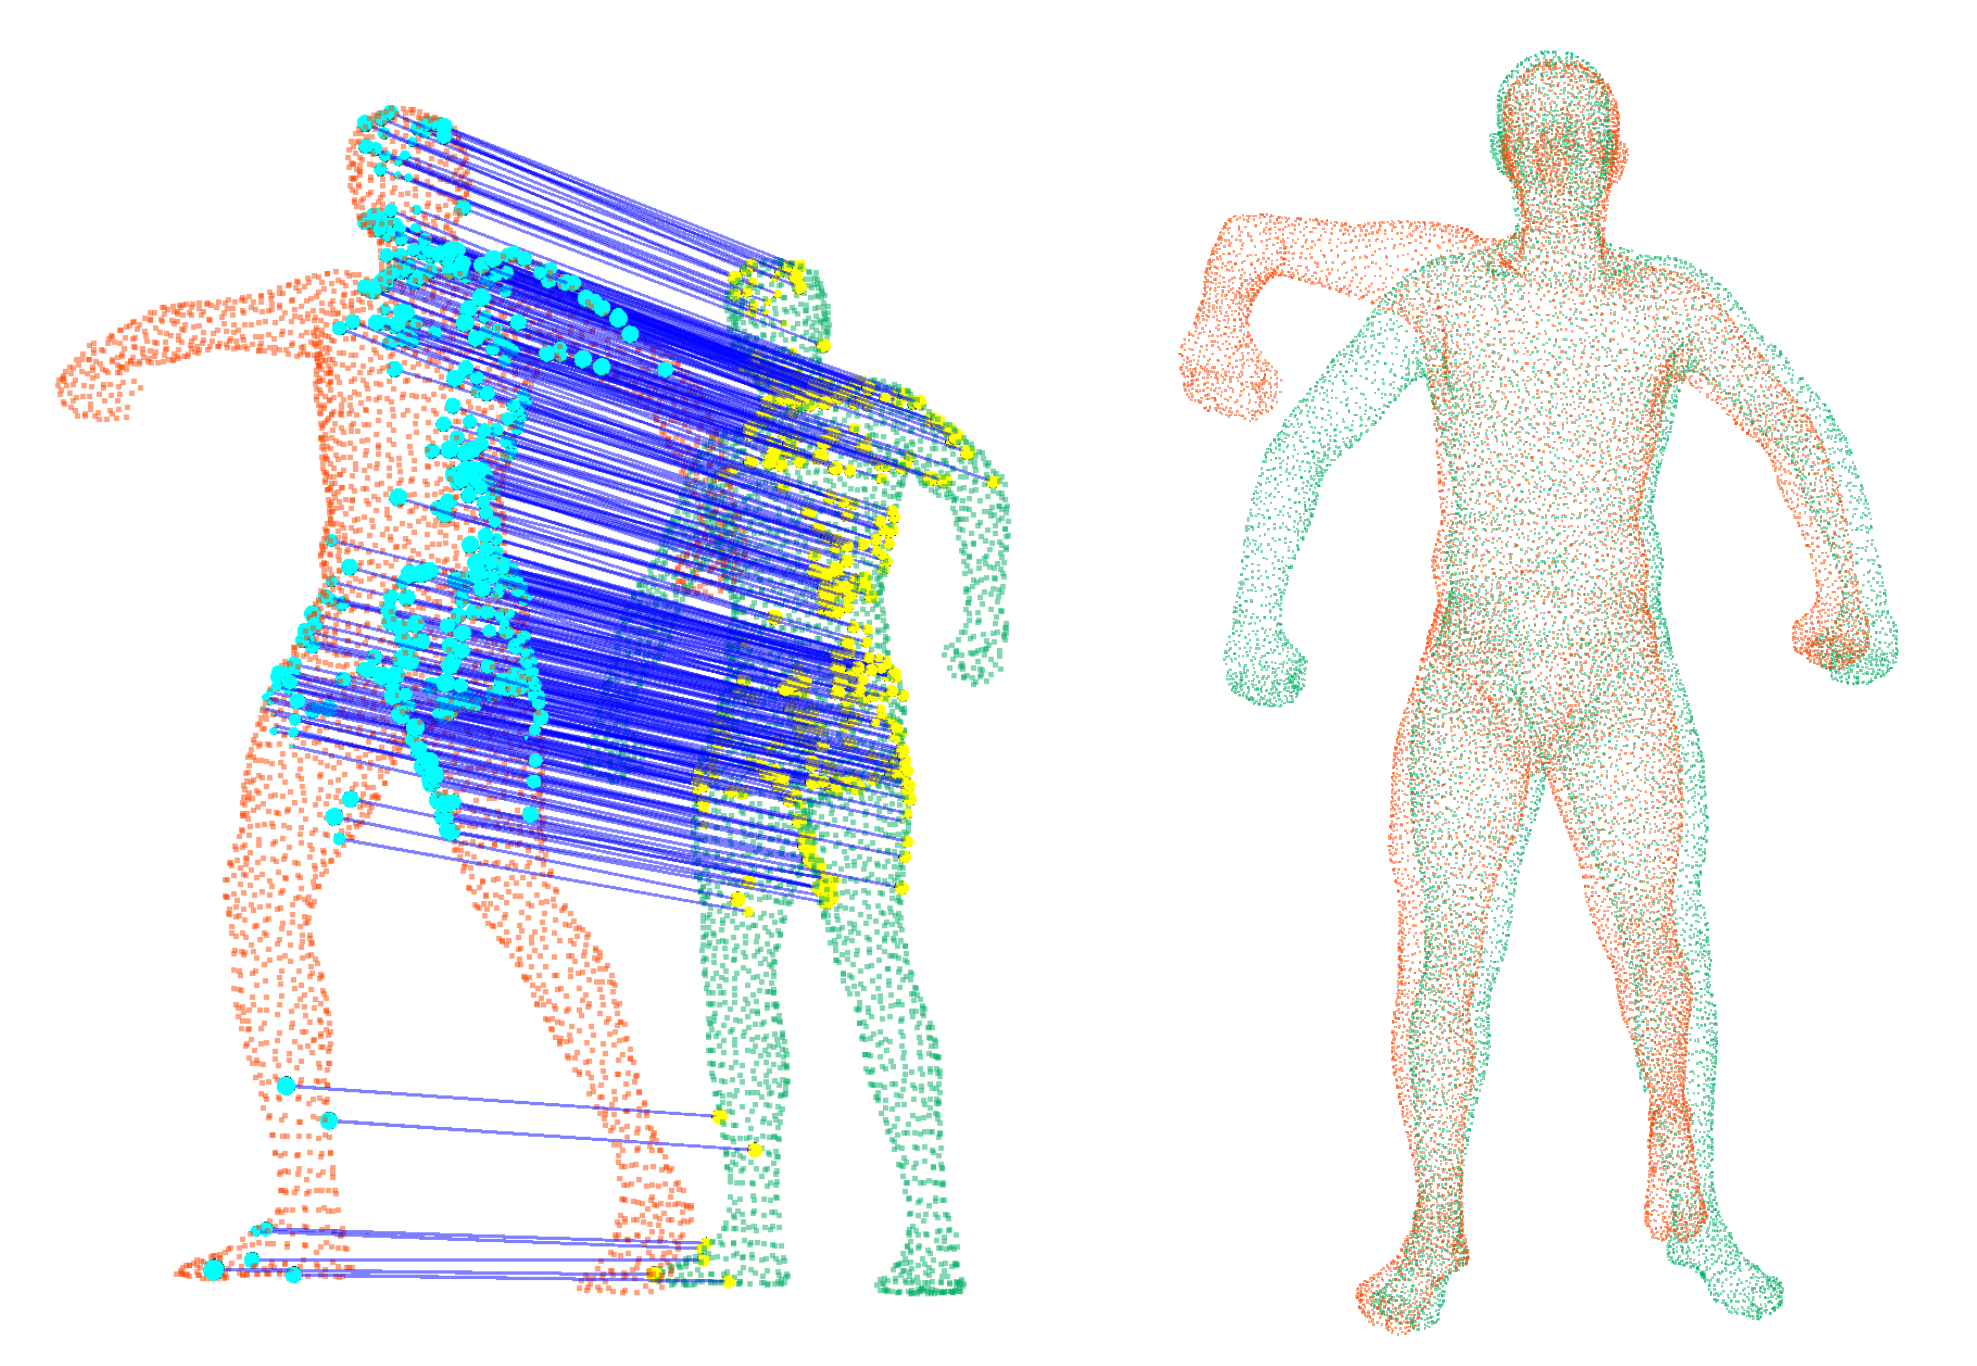
\includegraphics[width=0.45\textwidth]{LRP_body}} &		% JPEG file
		\fbox{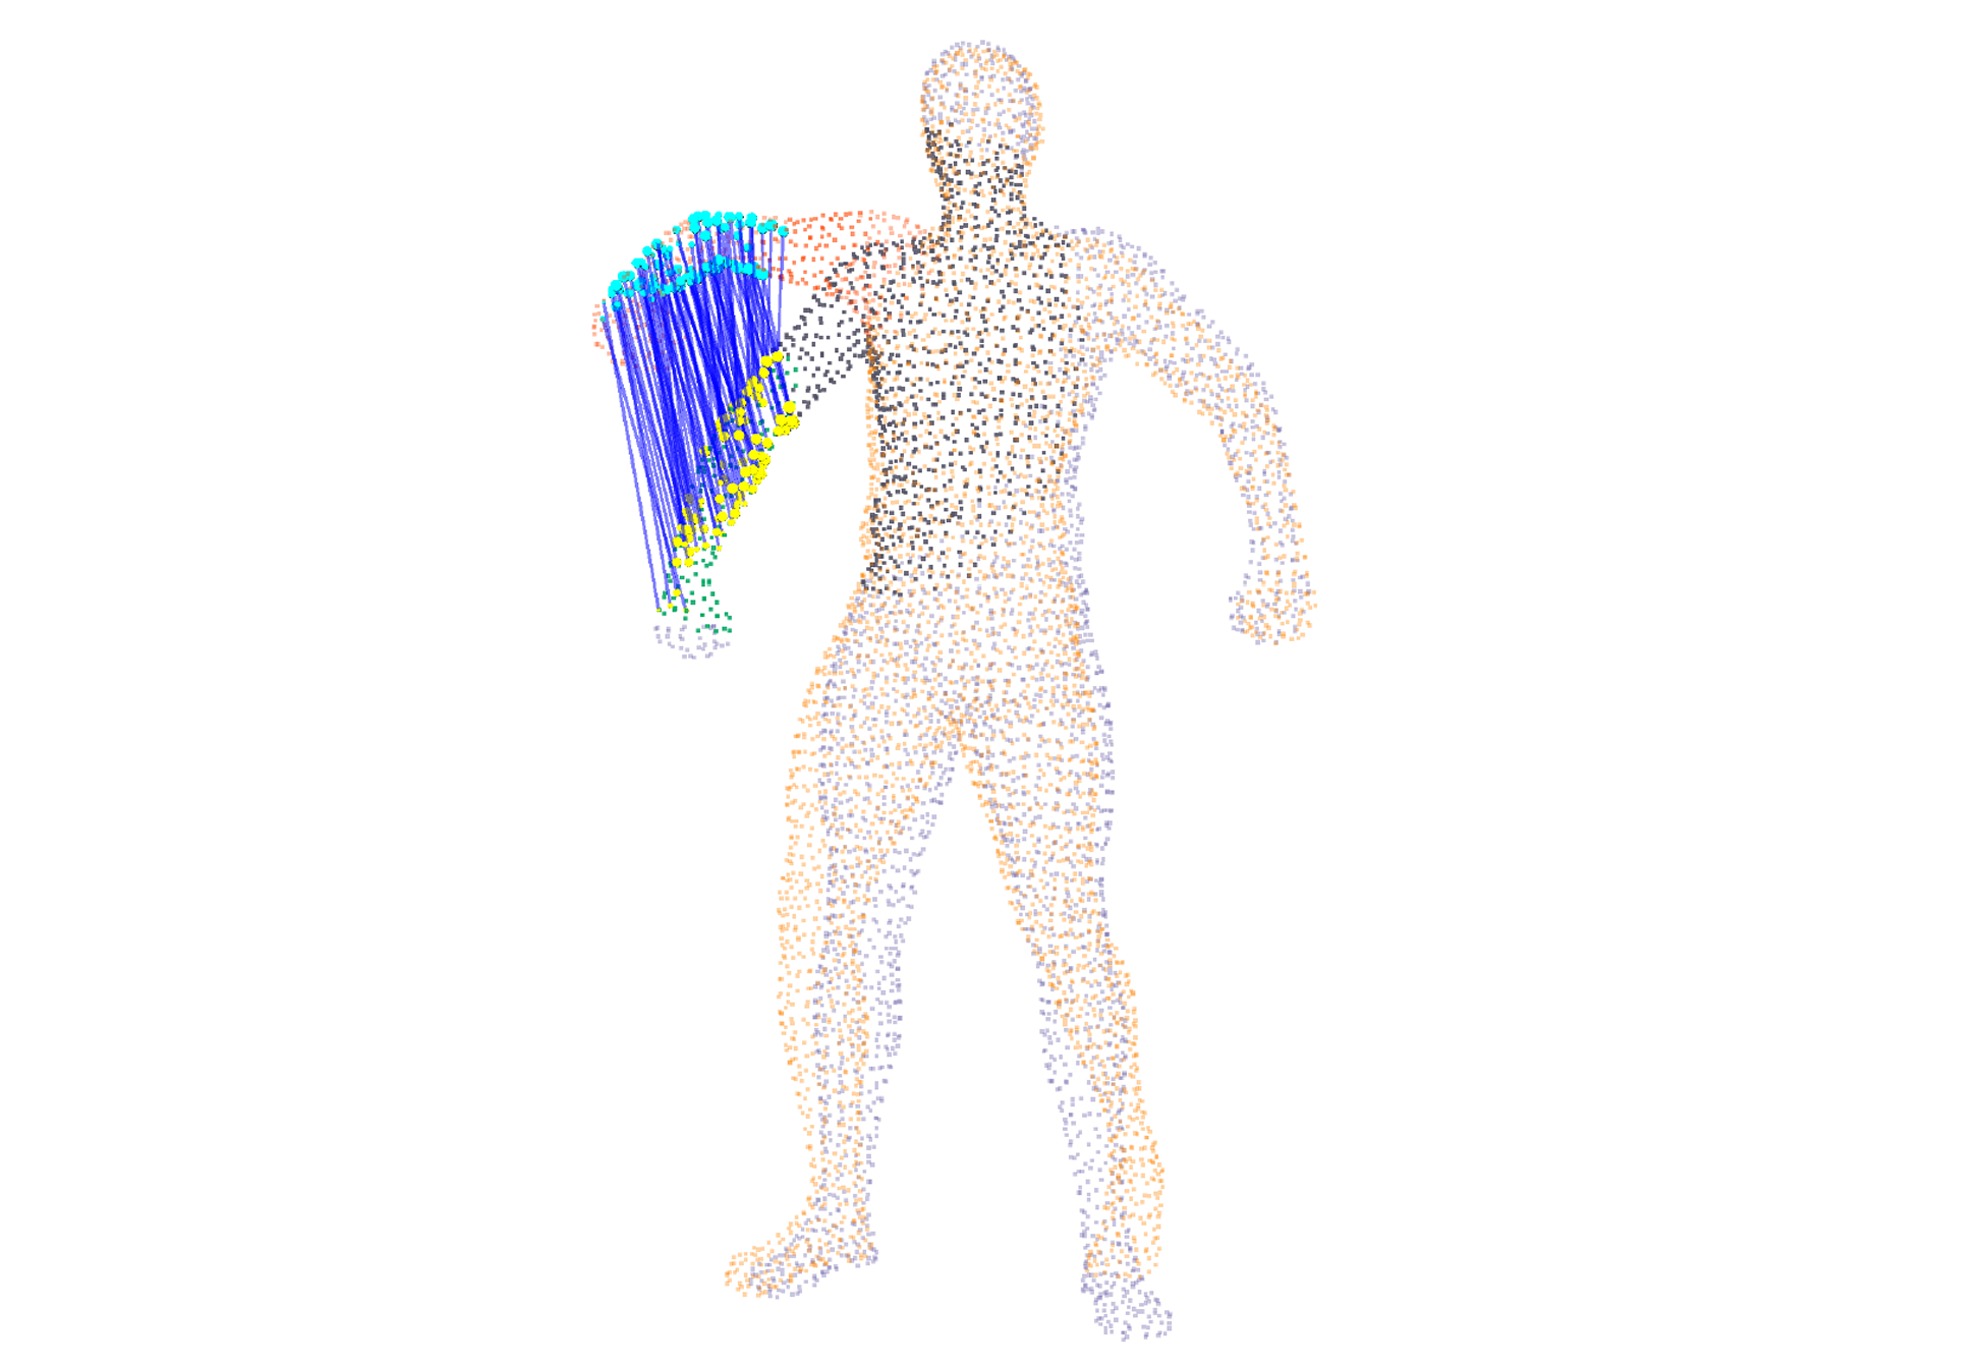
\includegraphics[width=0.45\textwidth]{LRP_arm}} 
		\\	% PNG file
		(a) & (b) 
	\end{tabular}
	\caption{Taking a mesh in two different poses as input (a), removing noise of the input point clouds (b)} 
	\label{fig:LRP_algorithm}
\end{figure}

\section{Registration}

Generally, registration means the alignment of rigid point clouds (see Figure XXX). The well-known approach is the iterative closest point.

\subsection{Iterative closest Point (ICP)}

It takes two meshes as input and iteratively aligns them by detecting the nearest neighbors. After registering, a matching error $e$ is achieved, which states the euclidean distance between associated points.

\subsection{Non-rigid Registration}

In case of two non non-rigid objects (e.g. a human in different poses which is composed of rigid parts) the ICP can't be applied as it would lead to high errors. To be able to match two objects, a segmentation into its rigid parts is required, where two associated parts are matched with the ICP.


\section{Related Work}
\label{cha:relatedWork}

A main approach for non-rigid registration is proposed by Anguelov \cite{Anguelov04} using the correlated correspondence algorithm \cite{CorrelatedCorrespondance}. A different approach is reached by Symmetrization \cite{Mitra07} and the recursive detection of body parts by the LRP -- ``largest rigid part'' algorithm \cite {guo2016correspondence}. Based on \cite{Anguelov04} and \cite{Mitra07}, Chang et al developed a closely related approach \cite{chang08articulated} \cite{chang09range}.

Mainly referenced are following approaches:

\subsection{Correlated Correspondence}

This algorithm takes a template Mesh and other Meshes in different configurations as input. It performs an probabilistic framework and Expectation-Maximization (EM) to iterate between finding a decomposition of template into rigid parts and finding
the part in the other meshes.

\begin{figure}[htbp]
	\centering\small
	\begin{tabular}{cc}
		\fbox{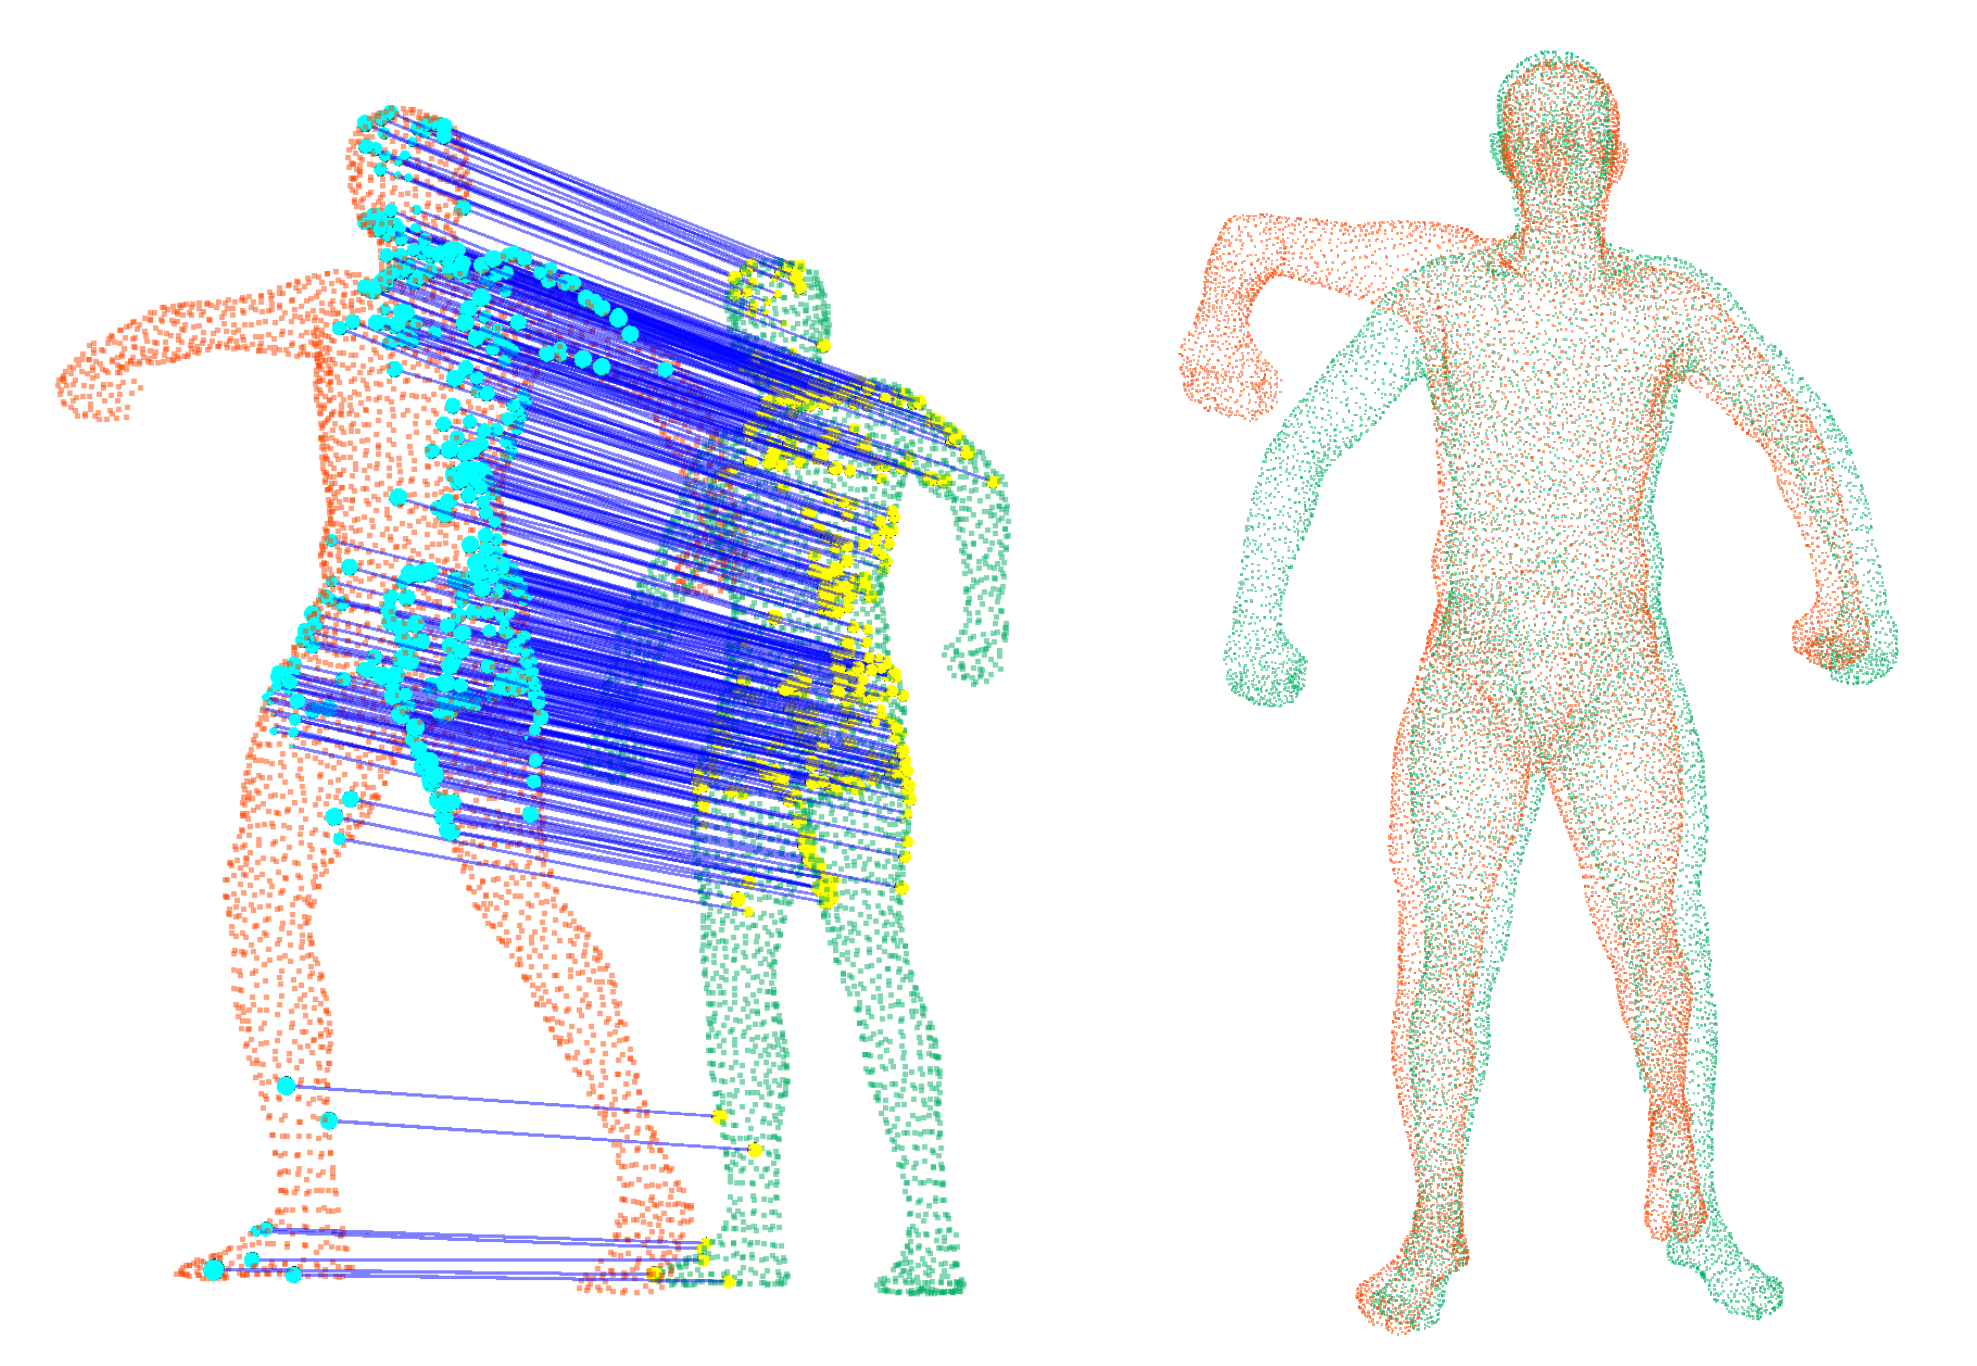
\includegraphics[width=0.45\textwidth]{LRP_body}} &		% JPEG file
		\fbox{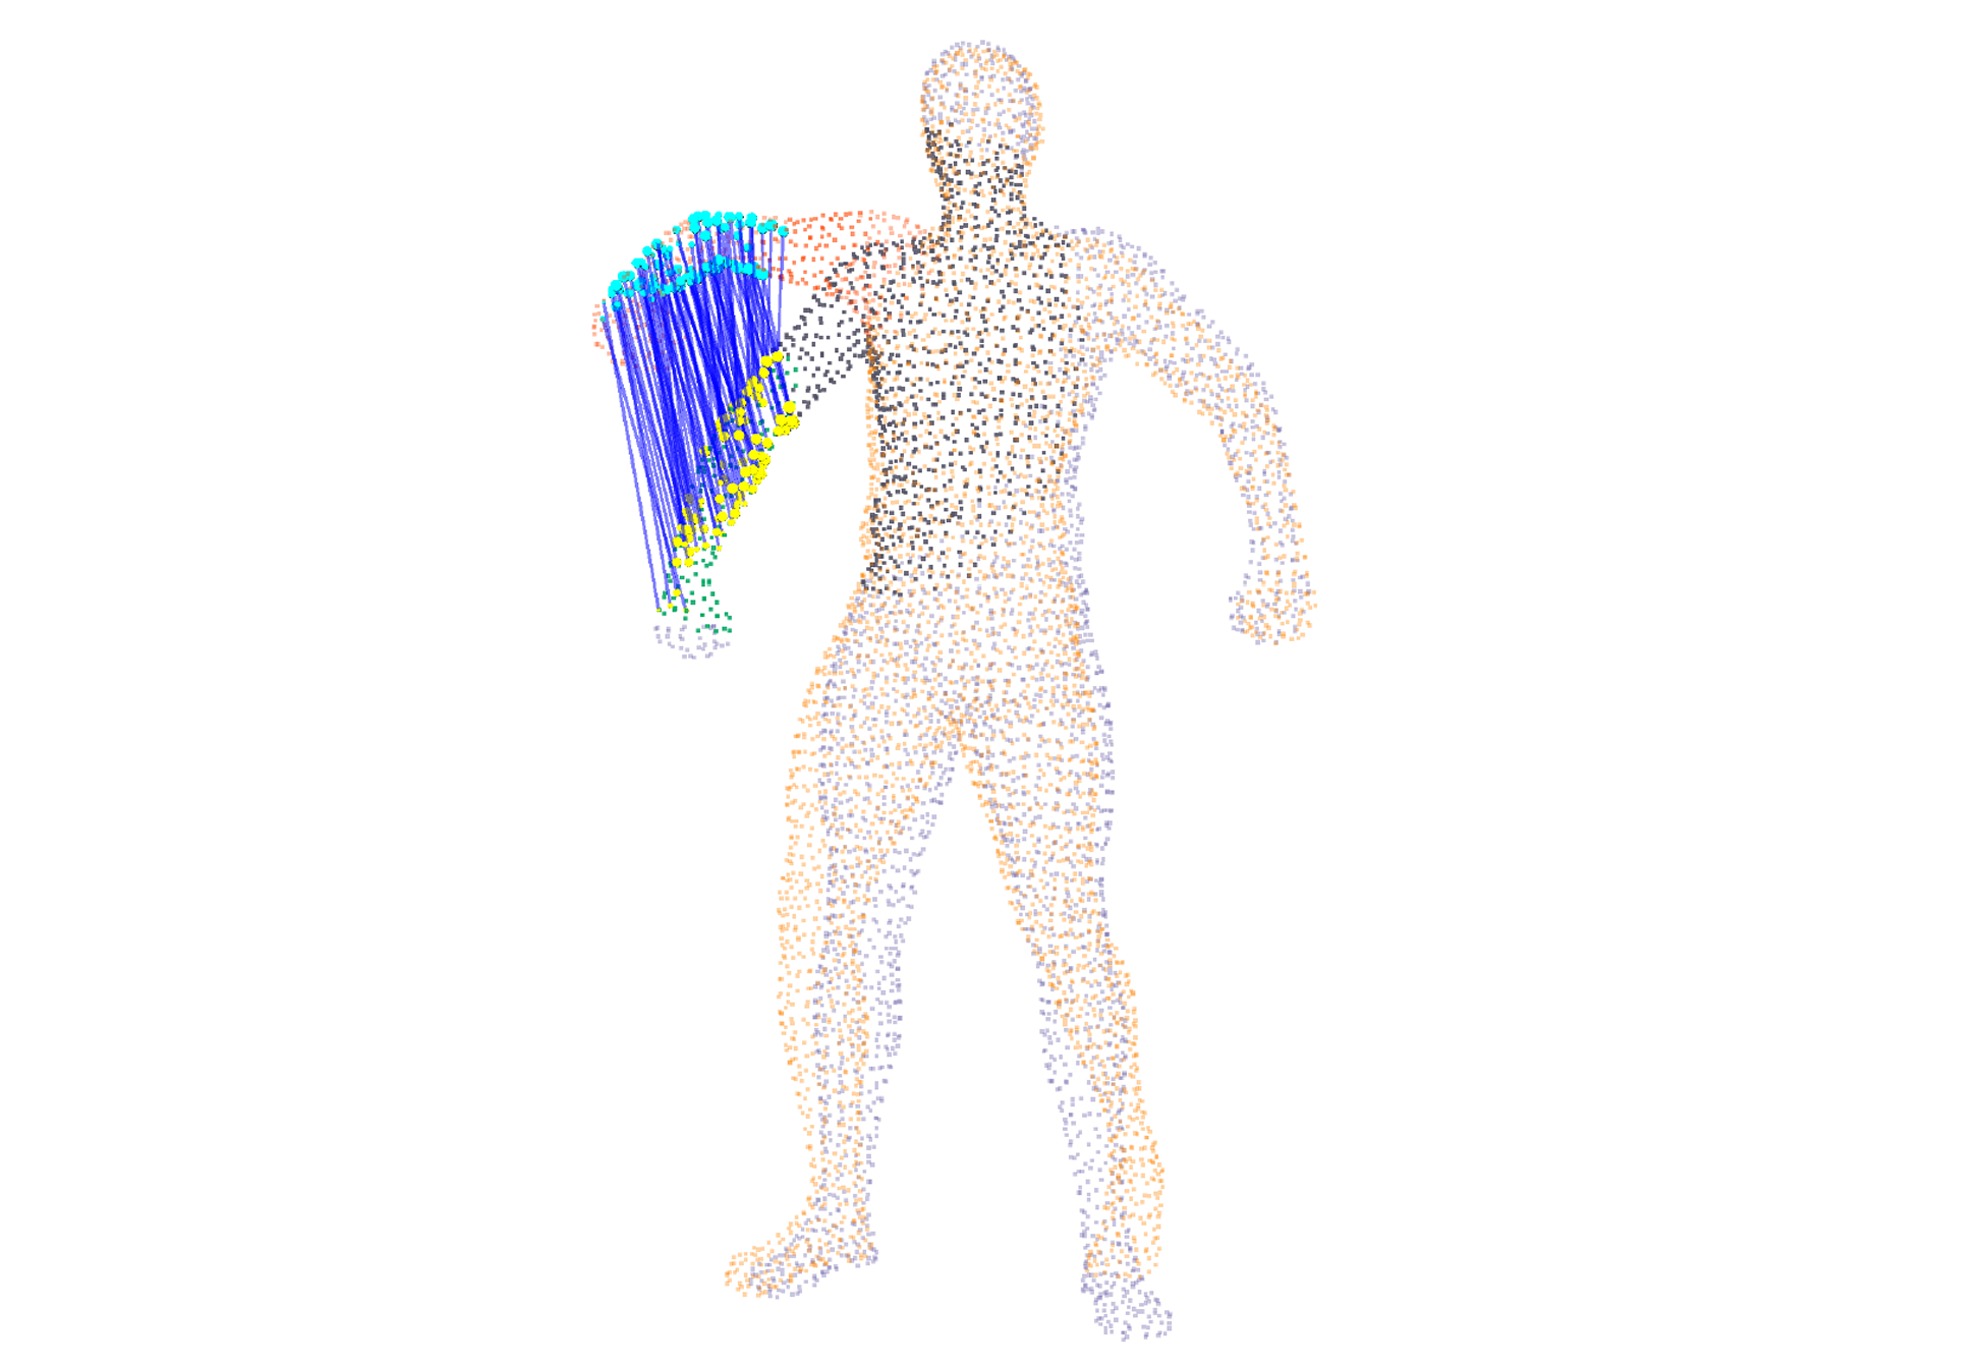
\includegraphics[width=0.45\textwidth]{LRP_arm}} 
		\\	% PNG file
		(a) & (b) 
	\end{tabular}
	\caption{Expectation-Maximization algorithm (a), to iteratively detect rigid parts (b)} 
	\label{fig:correlatedCorrespondence}
\end{figure}

\subsection{LRP}

The LRP algorithm discovers the articulated parts of two objects in different configurations by initially detecting the largest rigid part. This would be the biggest point cluster by applying a single rigid transformation. To reach that, sparse correspondences in combination with RANSAC are implemented. From there, the linking parts are recursively detected by growing clusters from the LRP and reapplying the algorithm. 

\begin{figure}[htbp]
	\centering\small
	\begin{tabular}{cc}
		\fbox{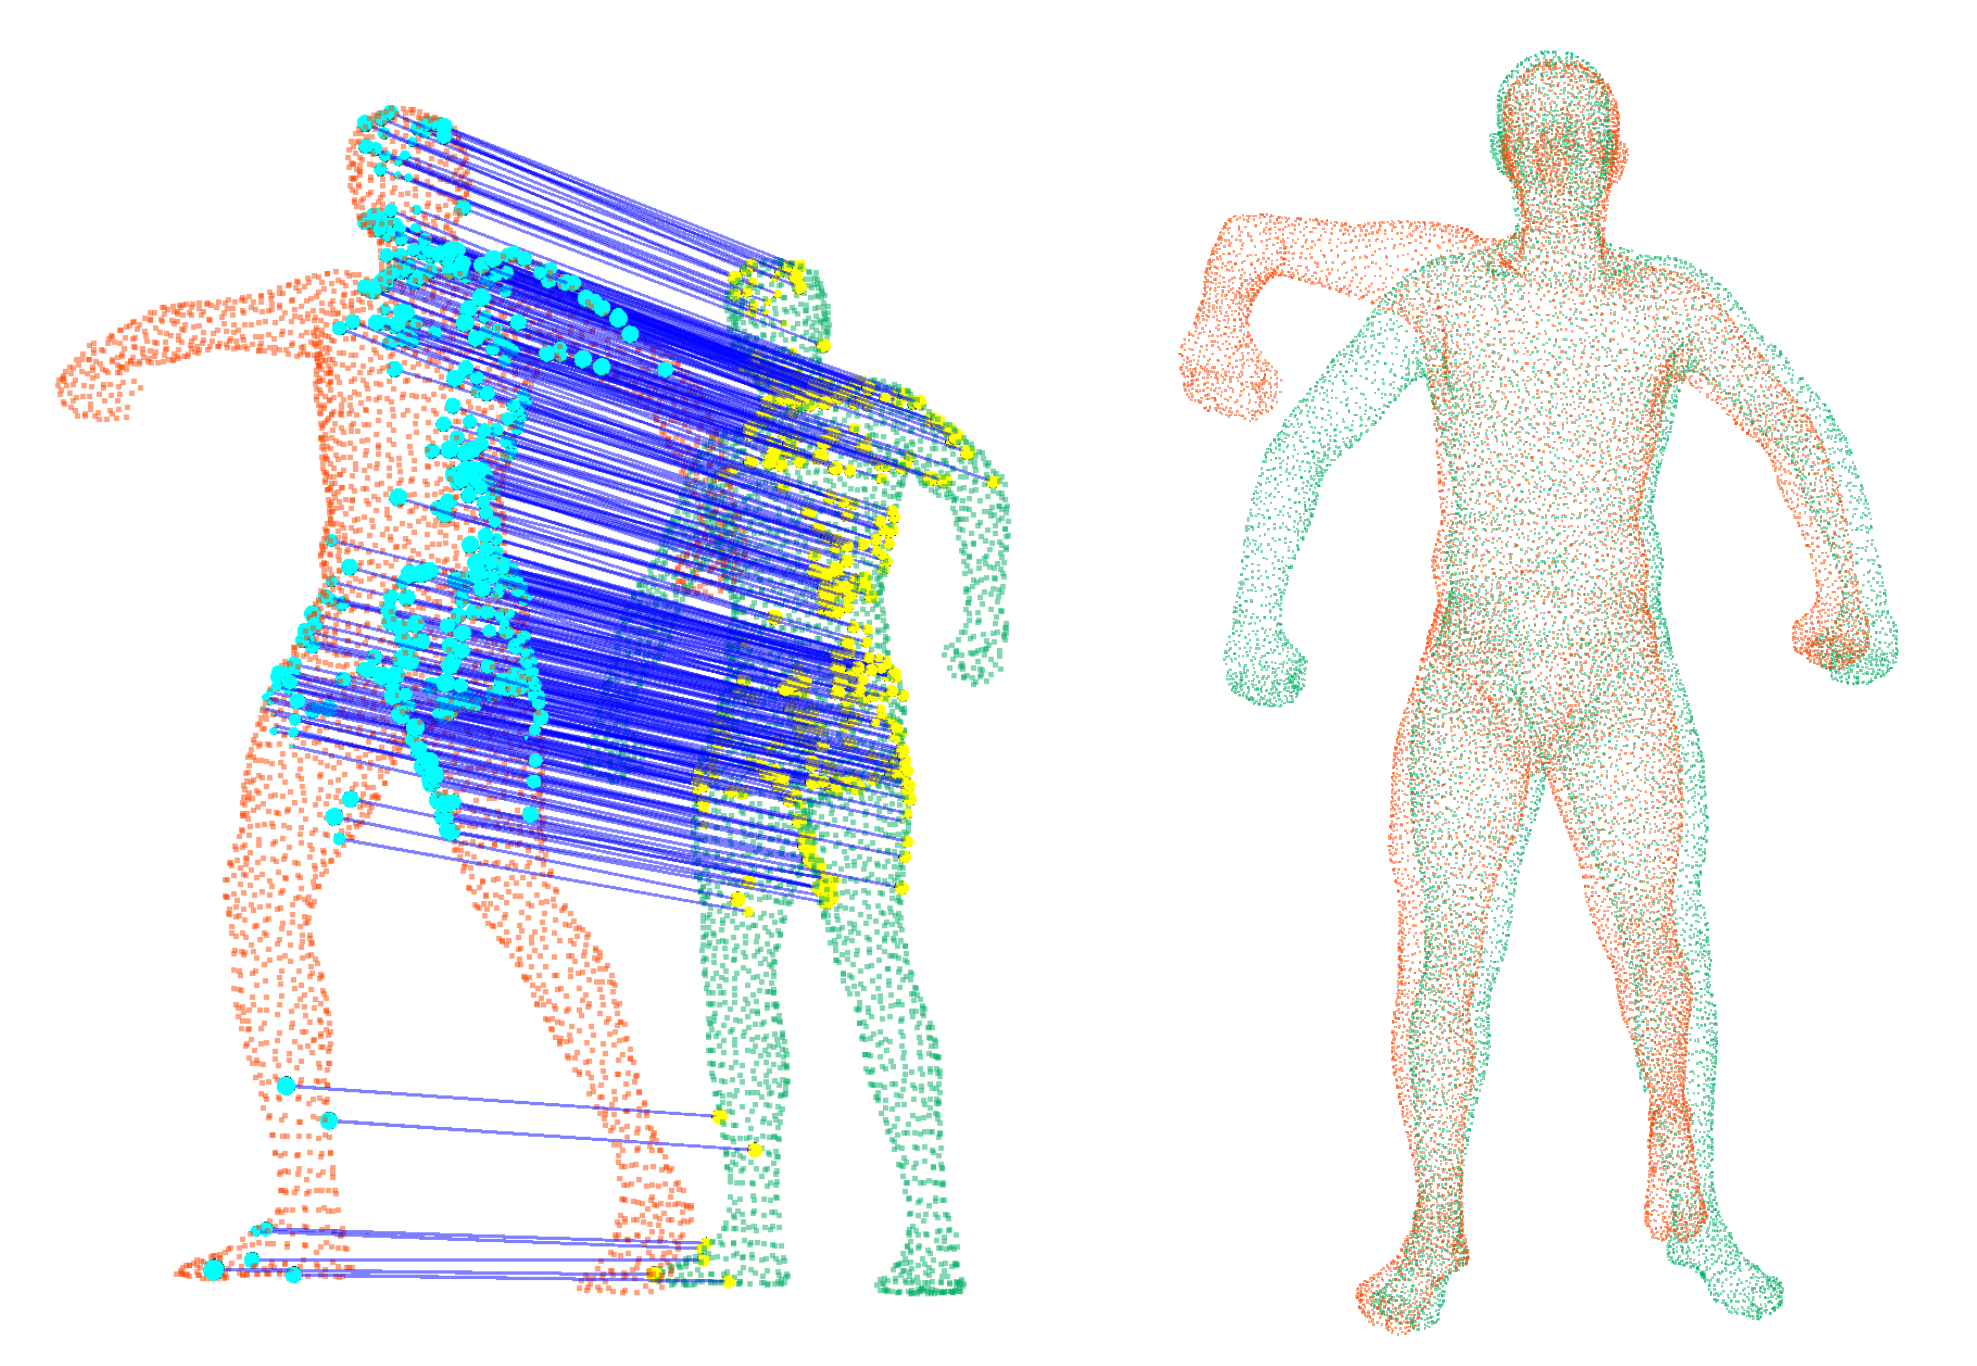
\includegraphics[width=0.45\textwidth]{LRP_body}} &		% JPEG file
		\fbox{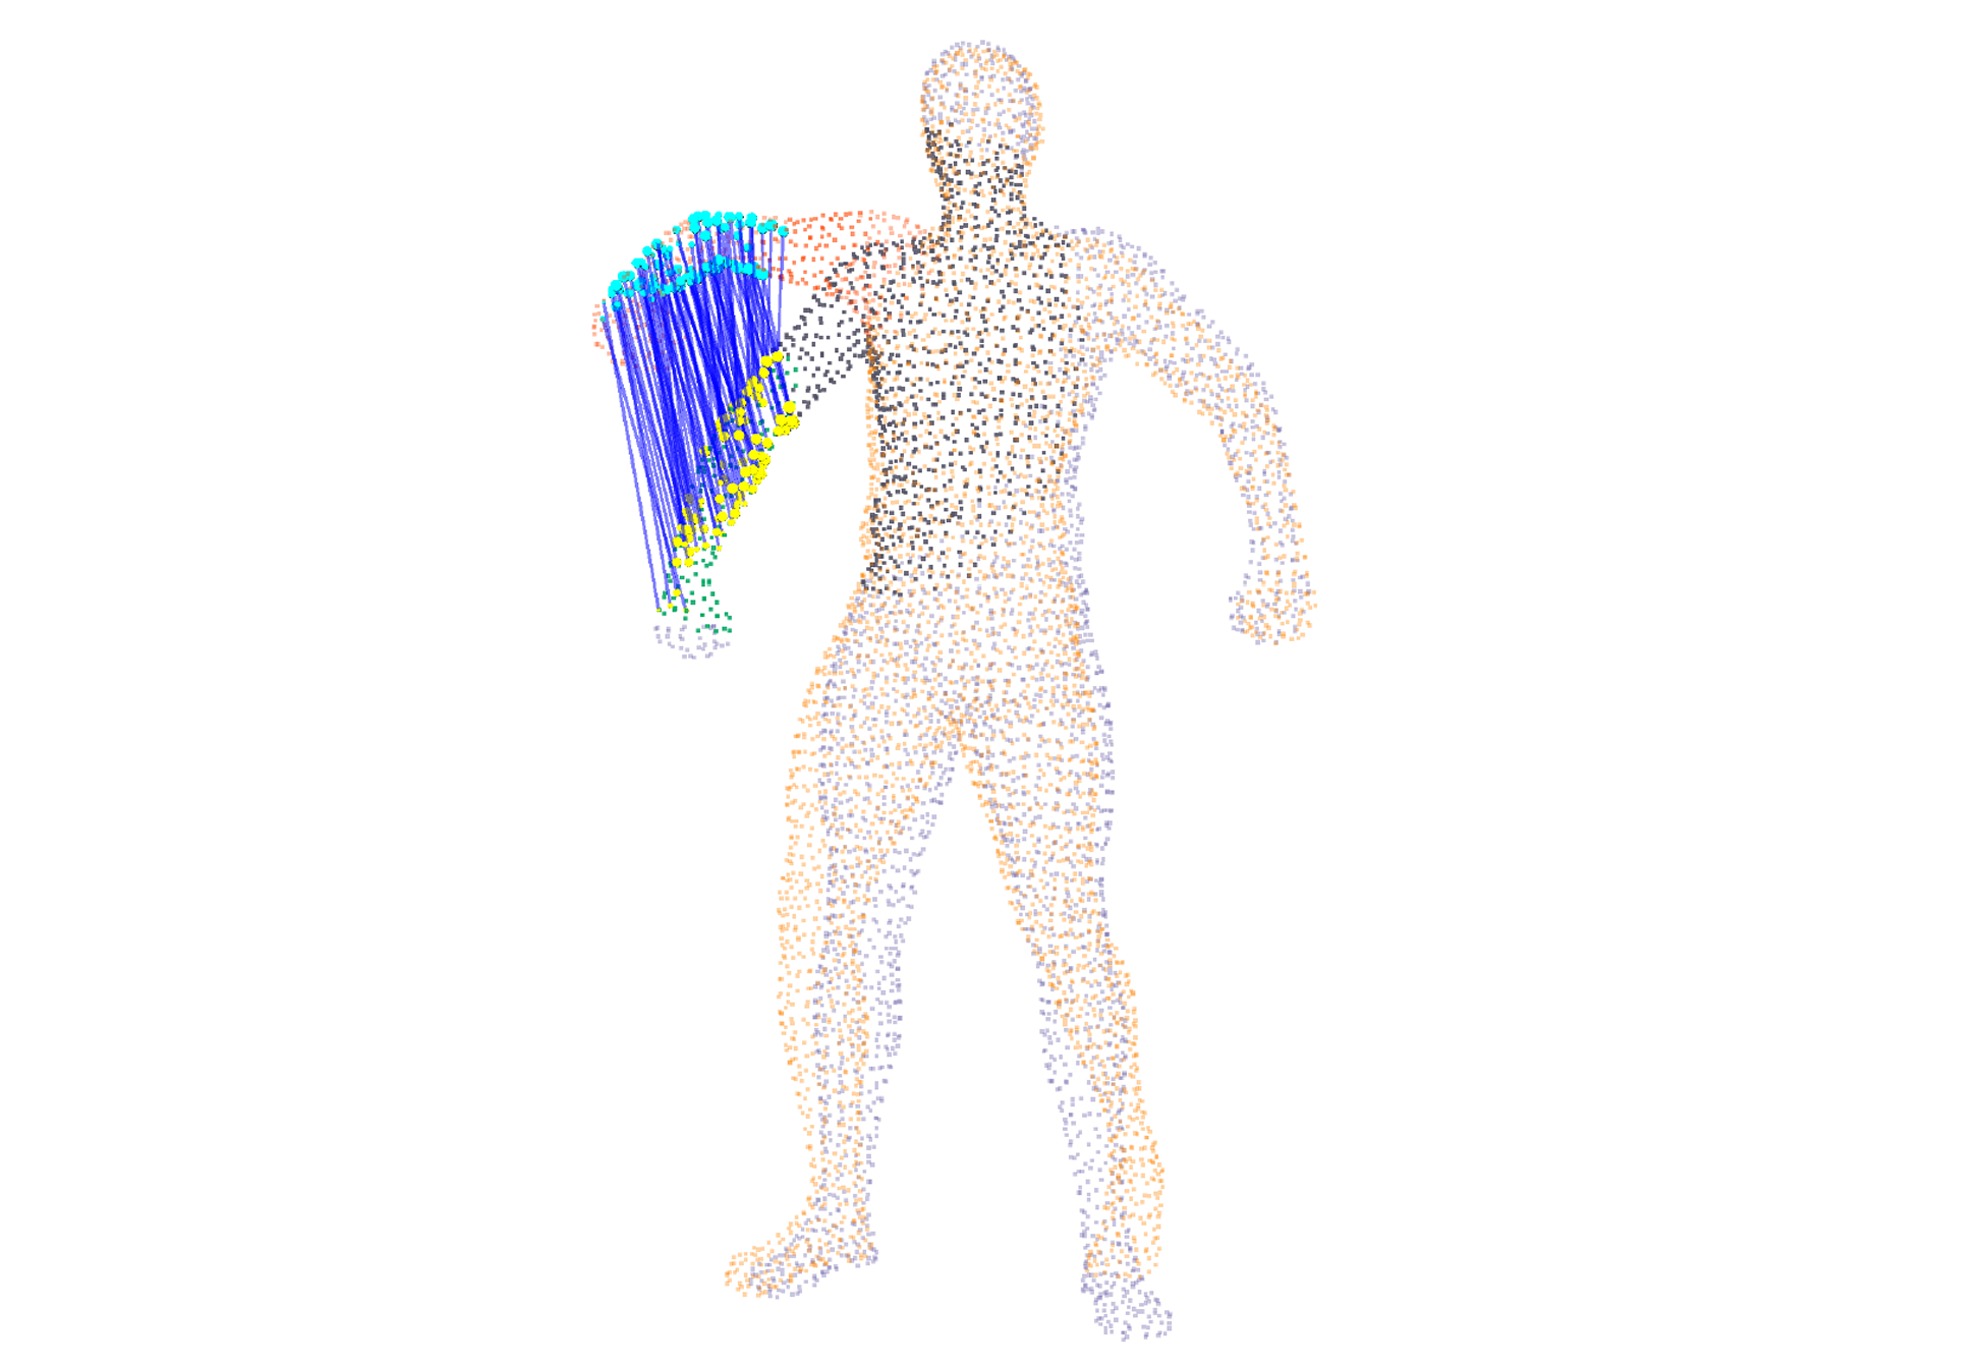
\includegraphics[width=0.45\textwidth]{LRP_arm}} 
		\\	% PNG file
		(a) & (b) 
	\end{tabular}
	\caption{Detecting the largest rigid part of an object (a), and align the object to recursively detect linking parts to the LRP (b)} 
	\label{fig:LRP_algorithm}
\end{figure}

\chapter{My contribution}
\label{cha:MyContribution}

This chapter focuses on the implementation of a new segmentation approach by taking the existing methods as reference (see section \ref{cha:relatedWork}). The algorithm has been first implemented in 2D, in order to be able to focus solely on developing and testing. Subsequently, it will be implemented in 3D using the PCL.

\section{Goal and approach}

The goal is to segment an articulated mesh $M$ into its unknown number $n$ of rigid parts $ P =  \{ {p_1,\ldots,p_n}\}$ and extract the joints $ J =  \{ {j_1,...,j_m}\}$ linking those parts in form of a skeleton structure. In general, this is done by non-rigid registration of the point clouds $S_0$ and $D_0$ of an object in two different poses. $S_0$ is thereby used as a \textit{template} to be registered with $D_0$. The main task is to determine a part assignment $p_i$ and the corresponding transformation $t_i$ for all points of the \textit{template} that alligns them with all points of $D_0$. Basically, a divide and conquer approach (see section \ref{divideAndConquer}) is implemented to recursively subdivide $S_0$ and $D_0$ into clusters trying to be matched. 

Problem?

\section{Assumptions}

The input mesh $M$ is assumed to solely consist of rigid parts that can not be deformed or stretched (e.g. rigid parts of a human) and are linked by joints. Comparing two poses $S_0$ and $D_0$ being adopted by the articulated object, the geodesic distance $g_{i,j}$ between two mesh points $p_i$ and $p_j$ remains constant. Thereby, it is taken advantage of the knowledge that points located on a rigid part $p_i$ have the same transformation $t_i$ . Furthermore, it is assumed that the two poses $S_0$ and $D_0$ of $M$ are oriented in the same direction.

Problem?

\section{Challenges/restrictions}

There are many challenges regarding the non-rigid registration of point clouds in 2D, as well as in 3D. First off, the input data can be noisy by means of points not belonging to the object. Furthermore, the approach is computationally expensive and time-consuming, as the corresponding body parts of two meshes need to be detected iteratively. Additionally, the inevitable difficulty of finding the global optimum, related to ambiguous body parts, has to be overcome.

\section{Approach}
\label{divideAndConquer}

Problems of other approaches

\subsection{General idea}

The algorithm starts with two sets of point clouds $S_0$ and $D_0$ of an object $M$ in different poses (see figure \ref{fig:pc_2parts}). The two point clouds are iteratively subdivided into point clusters $ C =  \{ {c_1, ... , c_m}\}$. In each iteration step two related clusters of $S_0$ and $D_0$ are matched by applying the ICP (iterative closest point) resulting in a matching error $e$. In case of $ e < \tau $, two clusters are assumed to match. Otherwise, the algorithm is applied recursively and the clusters are again subdivided into further clusters. The algorithm terminates if all resulting clusters of $S_0$ can be matched to all clusters of $D_0$. All neighboring clusters are then checked to be merged, in case of having divided a rigid part. After that step, the remaining clusters are assigned to rigid parts $ P =  \{ {p_1, ..., p_n}\}$.

\begin{figure}[htbp]
	\centering\small
	\begin{tabular}{cc}
		\fbox{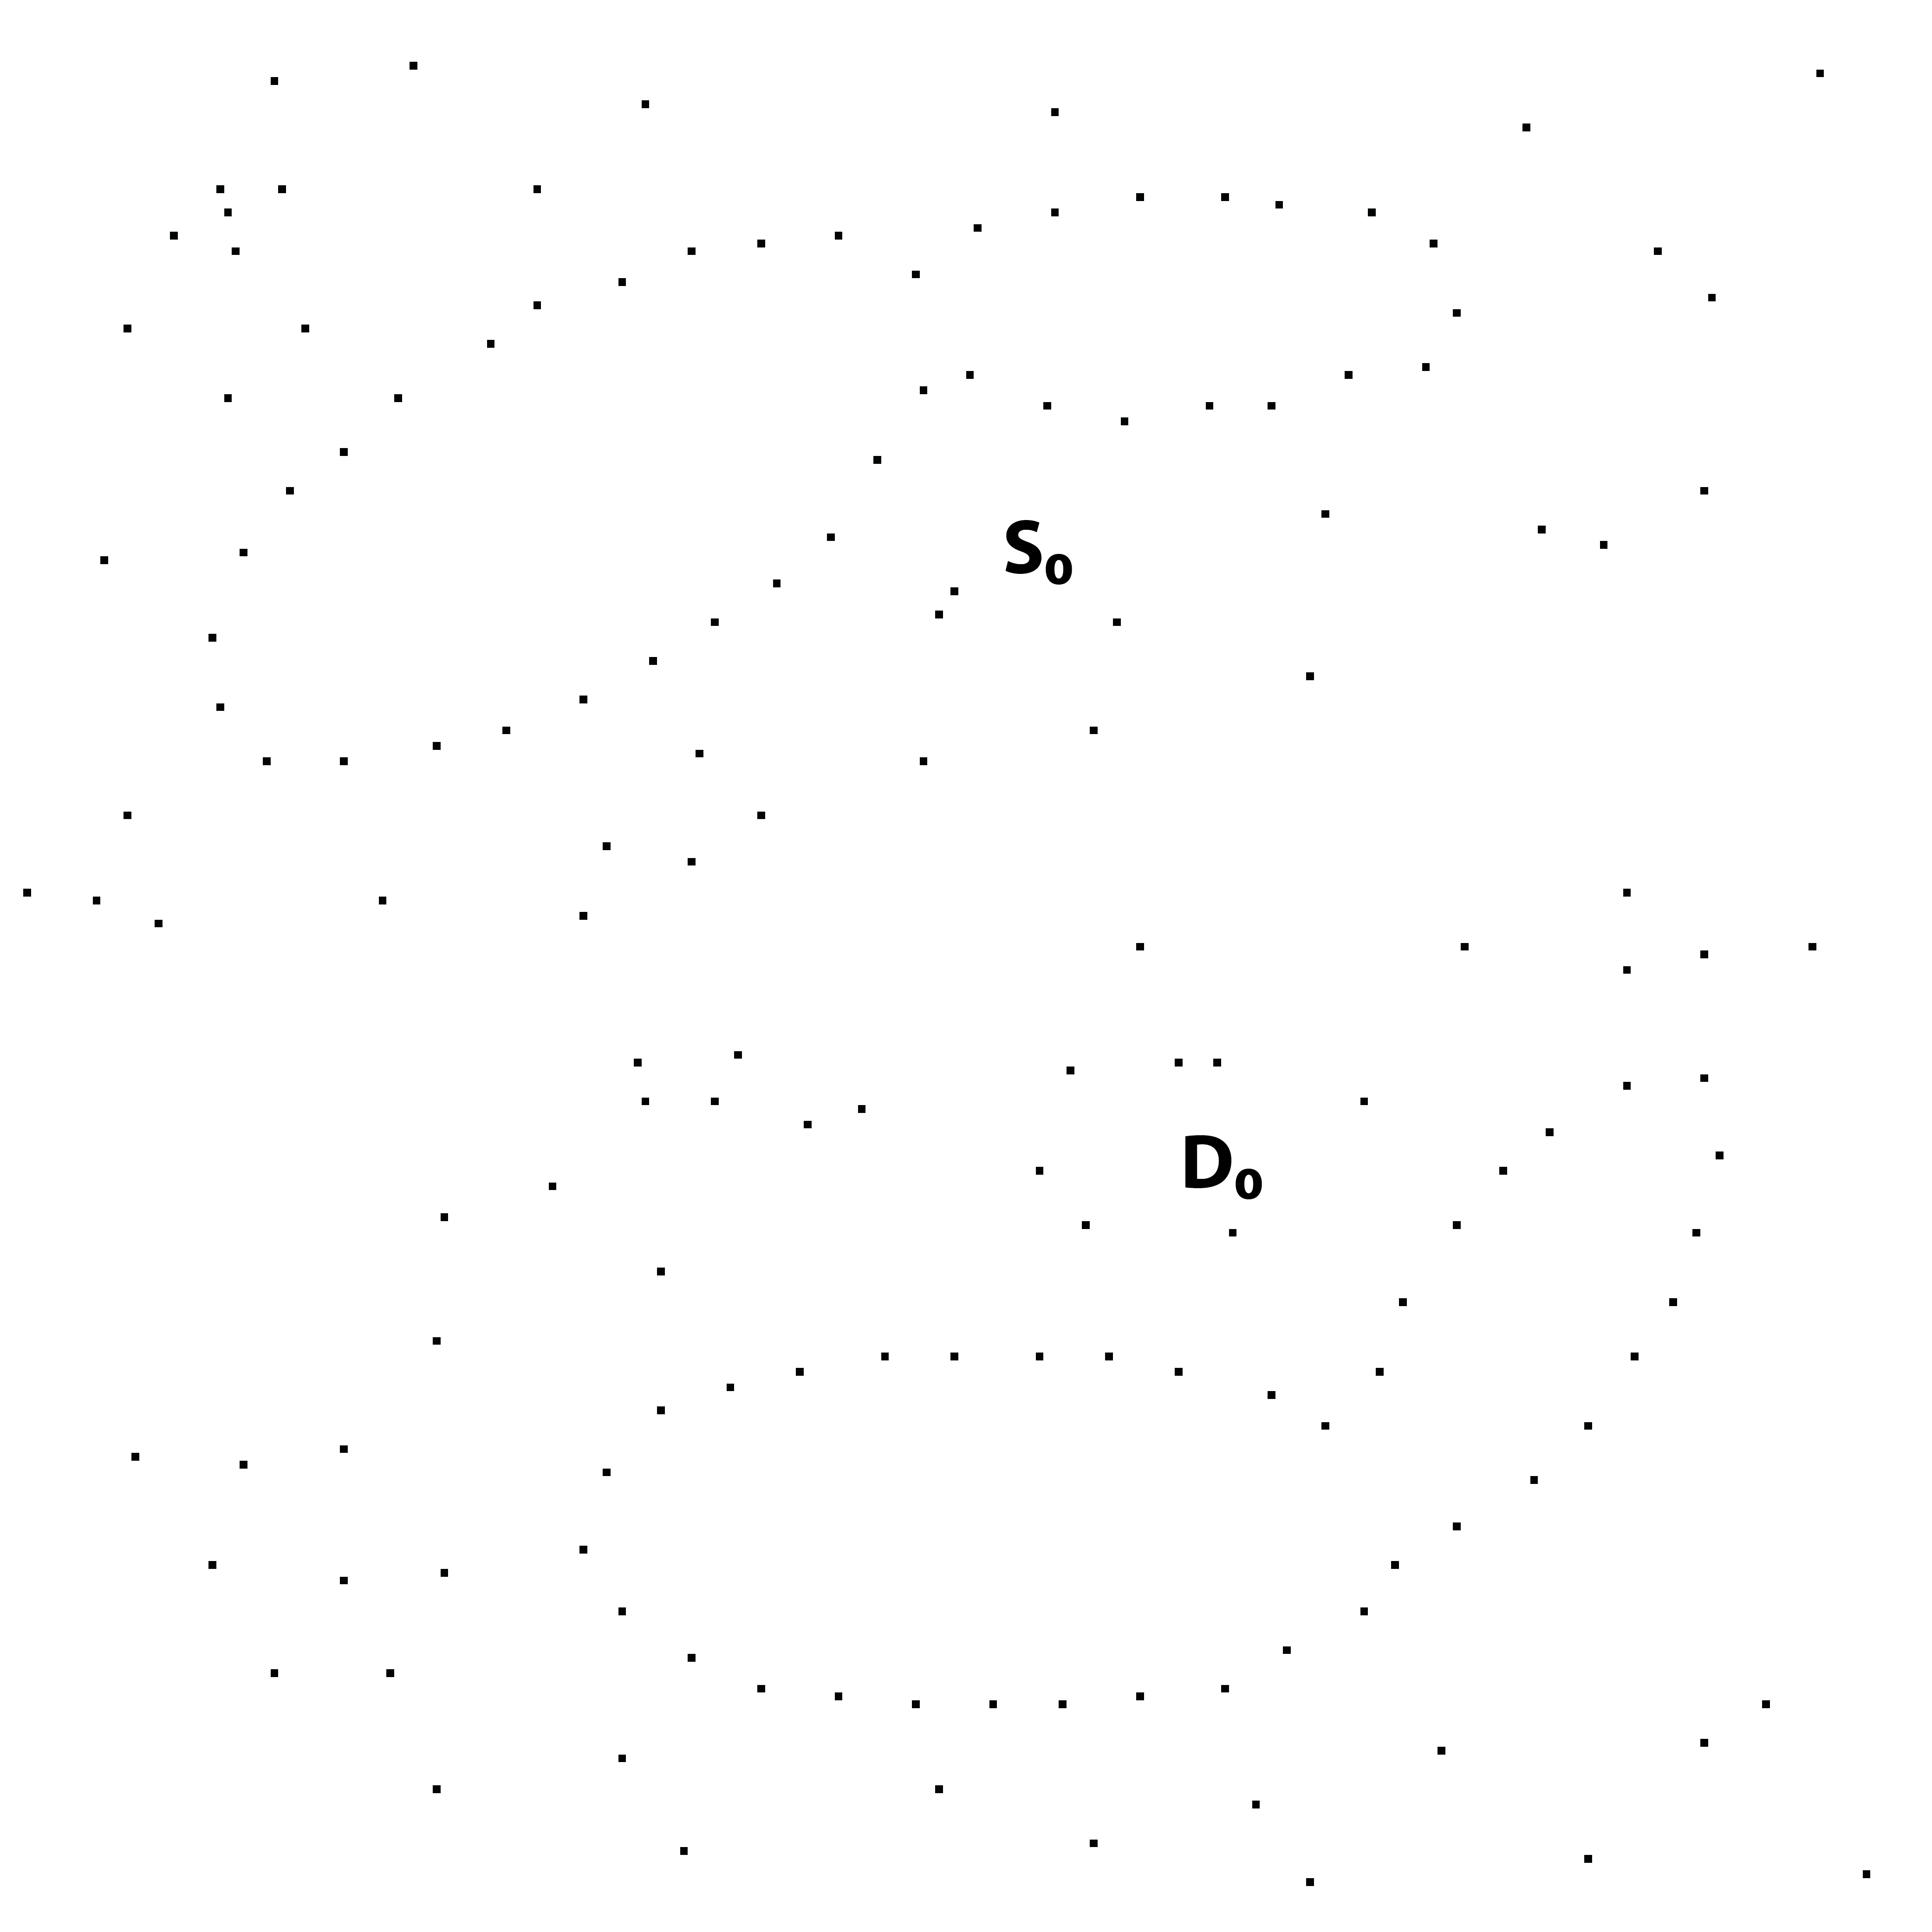
\includegraphics[width=0.45\textwidth]{pc_2parts_Noise}} &		% JPEG file
		\fbox{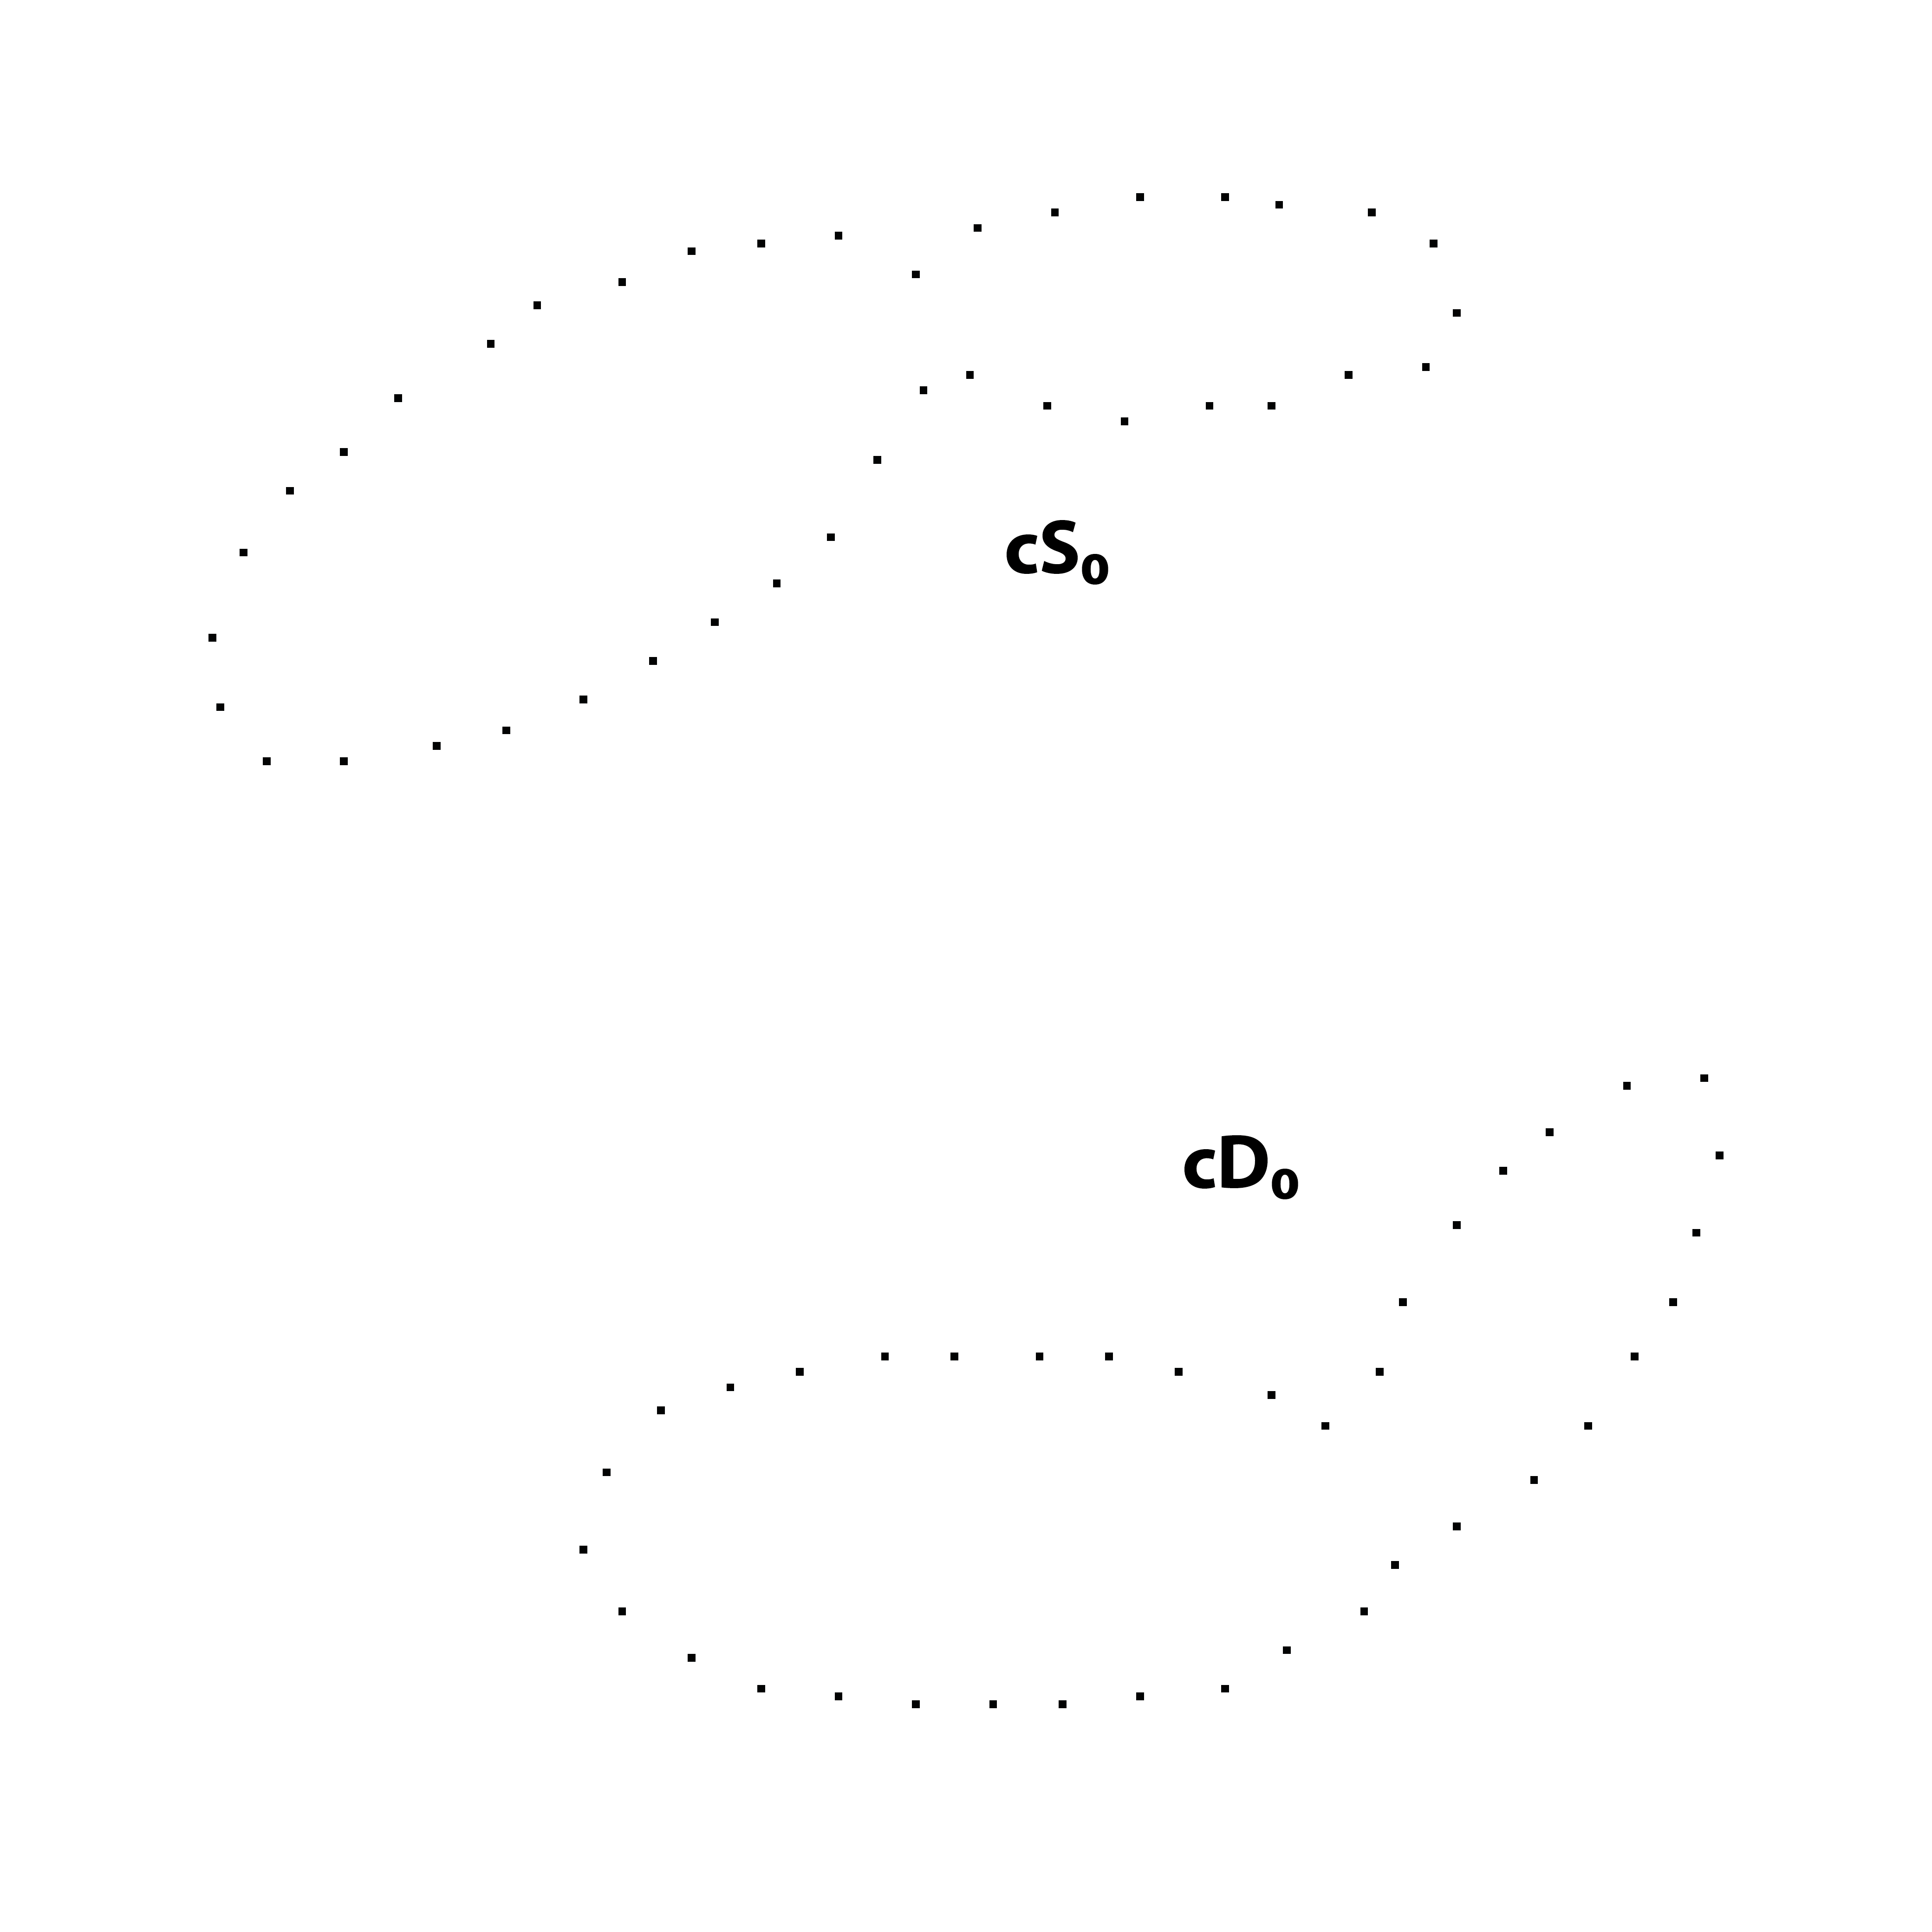
\includegraphics[width=0.45\textwidth]{pc_2parts_noNoise}} 
		\\	% PNG file
		(a) & (b) 
	\end{tabular}
	\caption{Taking a mesh in two different poses as input (a), removing noise of the input point clouds (b)} 
	\label{fig:pc_2parts}
\end{figure}

\subsection{Removing outliers}

As a first step, the outliers of the two point clouds $S_0$ and $D_0$ are removed. This is done, by detecting point clusters $\mathcal{C} = \{C_0, \ldots , C_m\}$. A cluster $c_i$ is grown from an unclustered point $\boldsymbol{p}_i$ of $S_0$ or $D_0$. Another point $p_j$ is added to the cluster $c_i$ if the euclidean distance between them $d(\boldsymbol{p}_i, \boldsymbol{p}_j)$ is below a pre-defined threshold $\tau$. All points of $c_i$ are then iteratively compared to the remaining unclustered points to allow the cluster to grow. Once, all points of $c_i$ have been treated, another unclustered point is used as a seed. If there are no unclustered points left, the clusters with the highest number of points $n$ are selected as input clusters $cS_0$ and $C_{1,0}$ (see figure \ref{fig:pc_2parts}).


\subsection{Subdividing into clusters}

As a next step, the two main clusters $cS_0$ and $cD_0$ are taken as input for further computation steps. If the matching between the two clusters does not suceed, they are subdivided into two clusters. In the other case, no subdividing is done and the procedure is repeated recursively for all clusters $C = \{{c_1, ..., c_m}\} $ of $cS_0$ until they can be matched to all clusters of $cD_0$   

\subsubsection{Divider position}

To determine where to divide a cluster, it is taken advantage of the PCA (principal component analysis). The resulting dividers $d_S$ and $d_D$ are realised by computing the principal axes $p_S$ and $p_D$ through the centroids $ct_0$ and taking the perpendicular secondary axes $s_S$ and $s_D$ through the centroids (see figure \ref{fig:dc_axes_2p}).

\begin{figure}
	\centering
	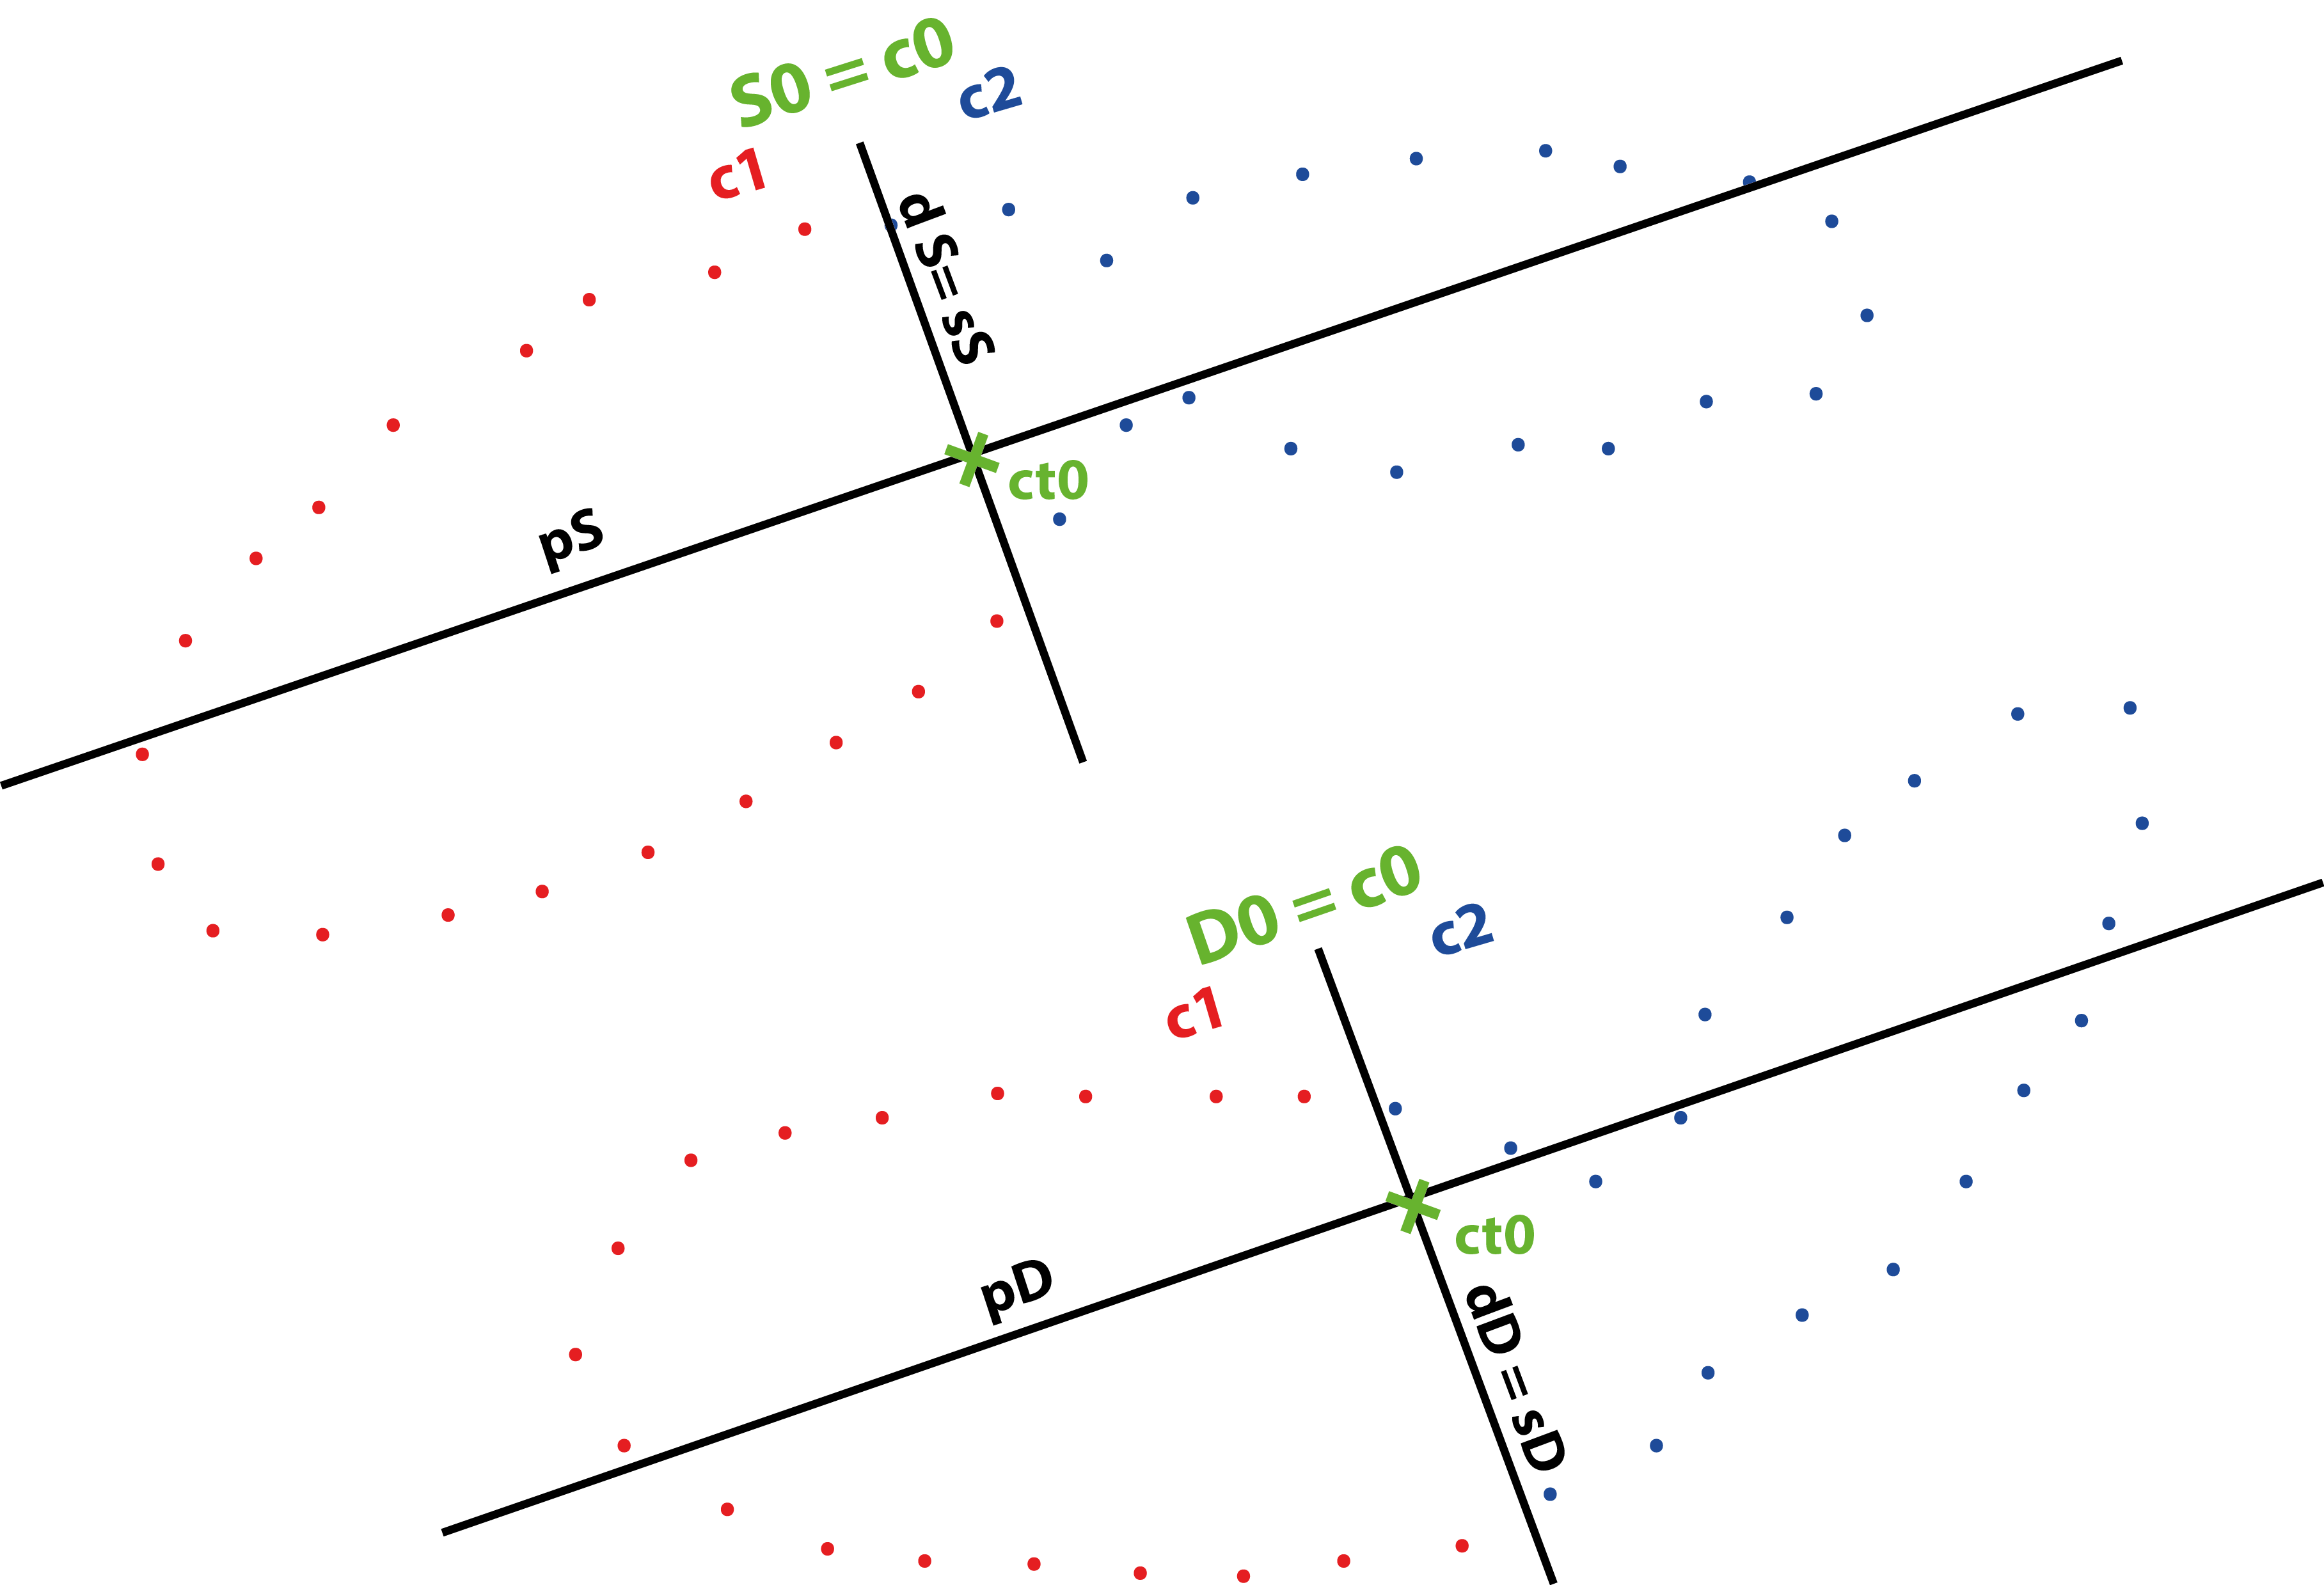
\includegraphics[width=0.7\linewidth]{illustration_axes}
	\caption{Dividing \textit{S\textsubscript{0}} and \textit{D\textsubscript{0}} into clusters by the divider \textit{d} to match them with ICP.}
	\label{fig:dc_axes_2p}
\end{figure}

\subsubsection{Declaring the matching condition between two clusters}

By applying the ICP and the nearest neighbour approach on two associated clusters $C_p$ and $C_q$, a certain matching error $e$ is computed between the cluster points blablabla $ C_p =  \{ p_0, \ldots, p_m\}$ and the associated points $ C_q =  \{ q_0, \ldots, q_m\}$. To make the matching error independent of the amount of cluster points, the average error per point $C_p, C_q$
%
\begin{equation}
	e_{\mathrm{avg}(C_p, C_q)} = \frac{1}{| C_p |} \cdot \displaystyle\sum_{i=0}^{m}\| \boldsymbol{p}_i - \boldsymbol{q}_i\|^2
\end{equation}
%
is computed, assuming that the two clusters $C_p$ and $C_q$ contain the same number of cluster points $m$. In case of different point amounts, the segmentation needs to be carried out at that clusters are always the same amount of points or some points are not considered during error amount calculation. To declare when two clusters match, it is quite essential to determine an appropriate threshold $\tau$. In case of being overvalued, clusters are more likely to be matched which could result in insufficient subdividing. On the other hand, the clusters are difficult to be matched, which will result in further subdividing and the detection of too many rigid parts. The two clusters $C_p$ are matching, if $e_{avg} < \tau$.

\subsubsection{Cluster tree}
\label{tree}

The subdividing of the clusters $cS_0$ and $cD_0$ is realised by a depth-first approach in a tree. Consequently, $cS_0$ and $cD_0$ are subdivided from the left to the right. A node $N$ of the tree contains two related clusters $cS_i$ of $S_0$ and $cS_i$ of $D_0$ and in case of subdividing it, a Node \textit{left}, containing the subdivided clusters $cS_{i+1}$ and $cD_{i+1}$, as well as a Node\textit{right}, containing the subdivided clusters $cS_{i+2}$ and $cD_{i+2}$. If two associated clusters \{$cS_{i+1}, cD_{i+1}$\} in a Node $N_i$ match, no further subdividing is performed. The resulting leaves of the tree are stored as matching clusters $C_l = \{{c_{l1}, ... , c_{lm}}\}$ (see figure \ref{fig:illustrationTree}). By applying the depth-first approach, the neighboring clusters in the list are also neighbouring clusters in the main clusters $cS_0$ or $cD_0$.  As a result, in the following steps the skeleton structure from an object can be extracted, where parts are connected by joints.

\begin{figure}
	\centering
	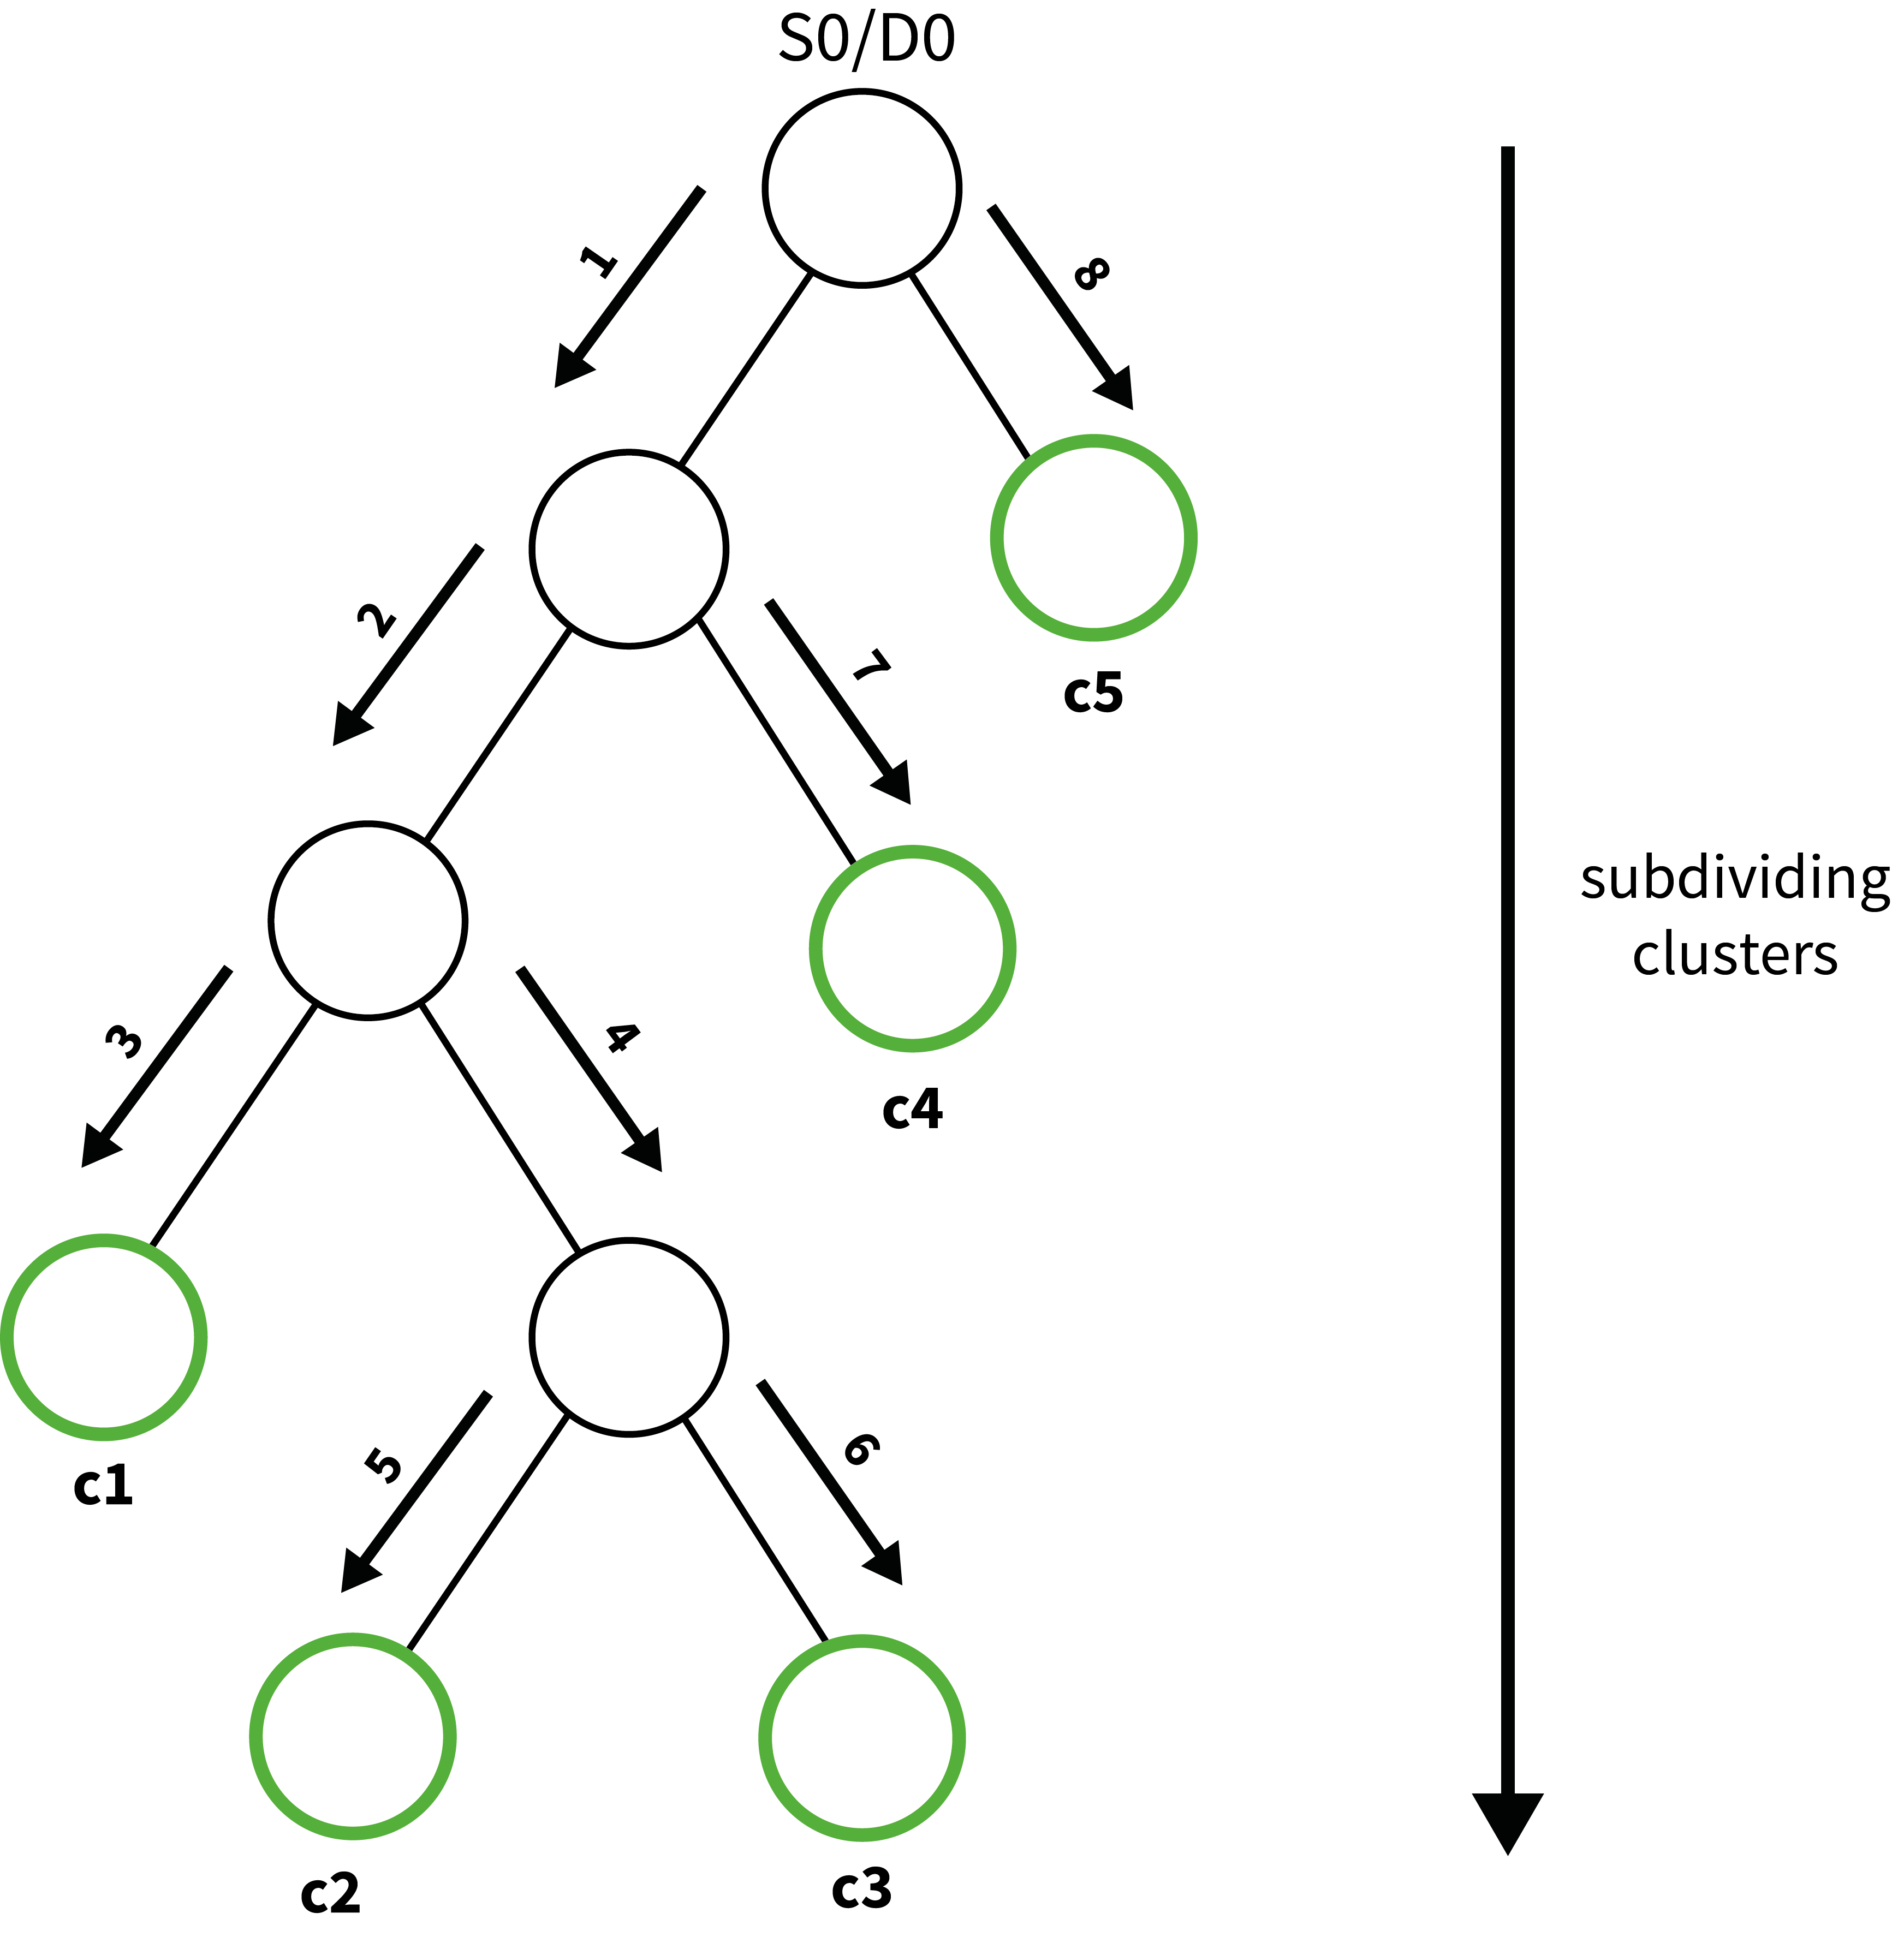
\includegraphics[width=0.7\linewidth]{IllustrationTree}
	\caption{Subdividing of S0 and D0 into matching clusters by the depth-first approach}
	\label{fig:illustrationTree}
\end{figure}

\subsection{Merging neighboring clusters to rigid parts}

As a next step, neighboring clusters from $C_l$ are iteratively merged and subsequently verified to match. This process is required to rejoin, if necessary, detected sub clusters to the rigid parts of the object. This is the case, if during the subdividing process, a rigid part was subdivided. The merging initiates with the first cluster $c_{li} = c_{l1}$ and its adjacent cluster $c_{li+1}$. If the resulting merged clusters $c_{ri} = c_{r1}$ can be matched, the merging proceeds with $c_{ri}$ and the adjacent cluster $c_{li+2}$. If not, the merging is not executed and $c_{li}$ is stored in a list of resulting clusters $C_r$. The whole procedure then starts with $c_{li+1}$. The process terminates if all clusters of $C_l$ are verified and consequently the clusters of $C_r$ are assigned to rigid parts $ P =  \{ {p_1,....p_n}\}$ (see figure \ref{fig:clusterChain}). 

\begin{figure}
	\centering
	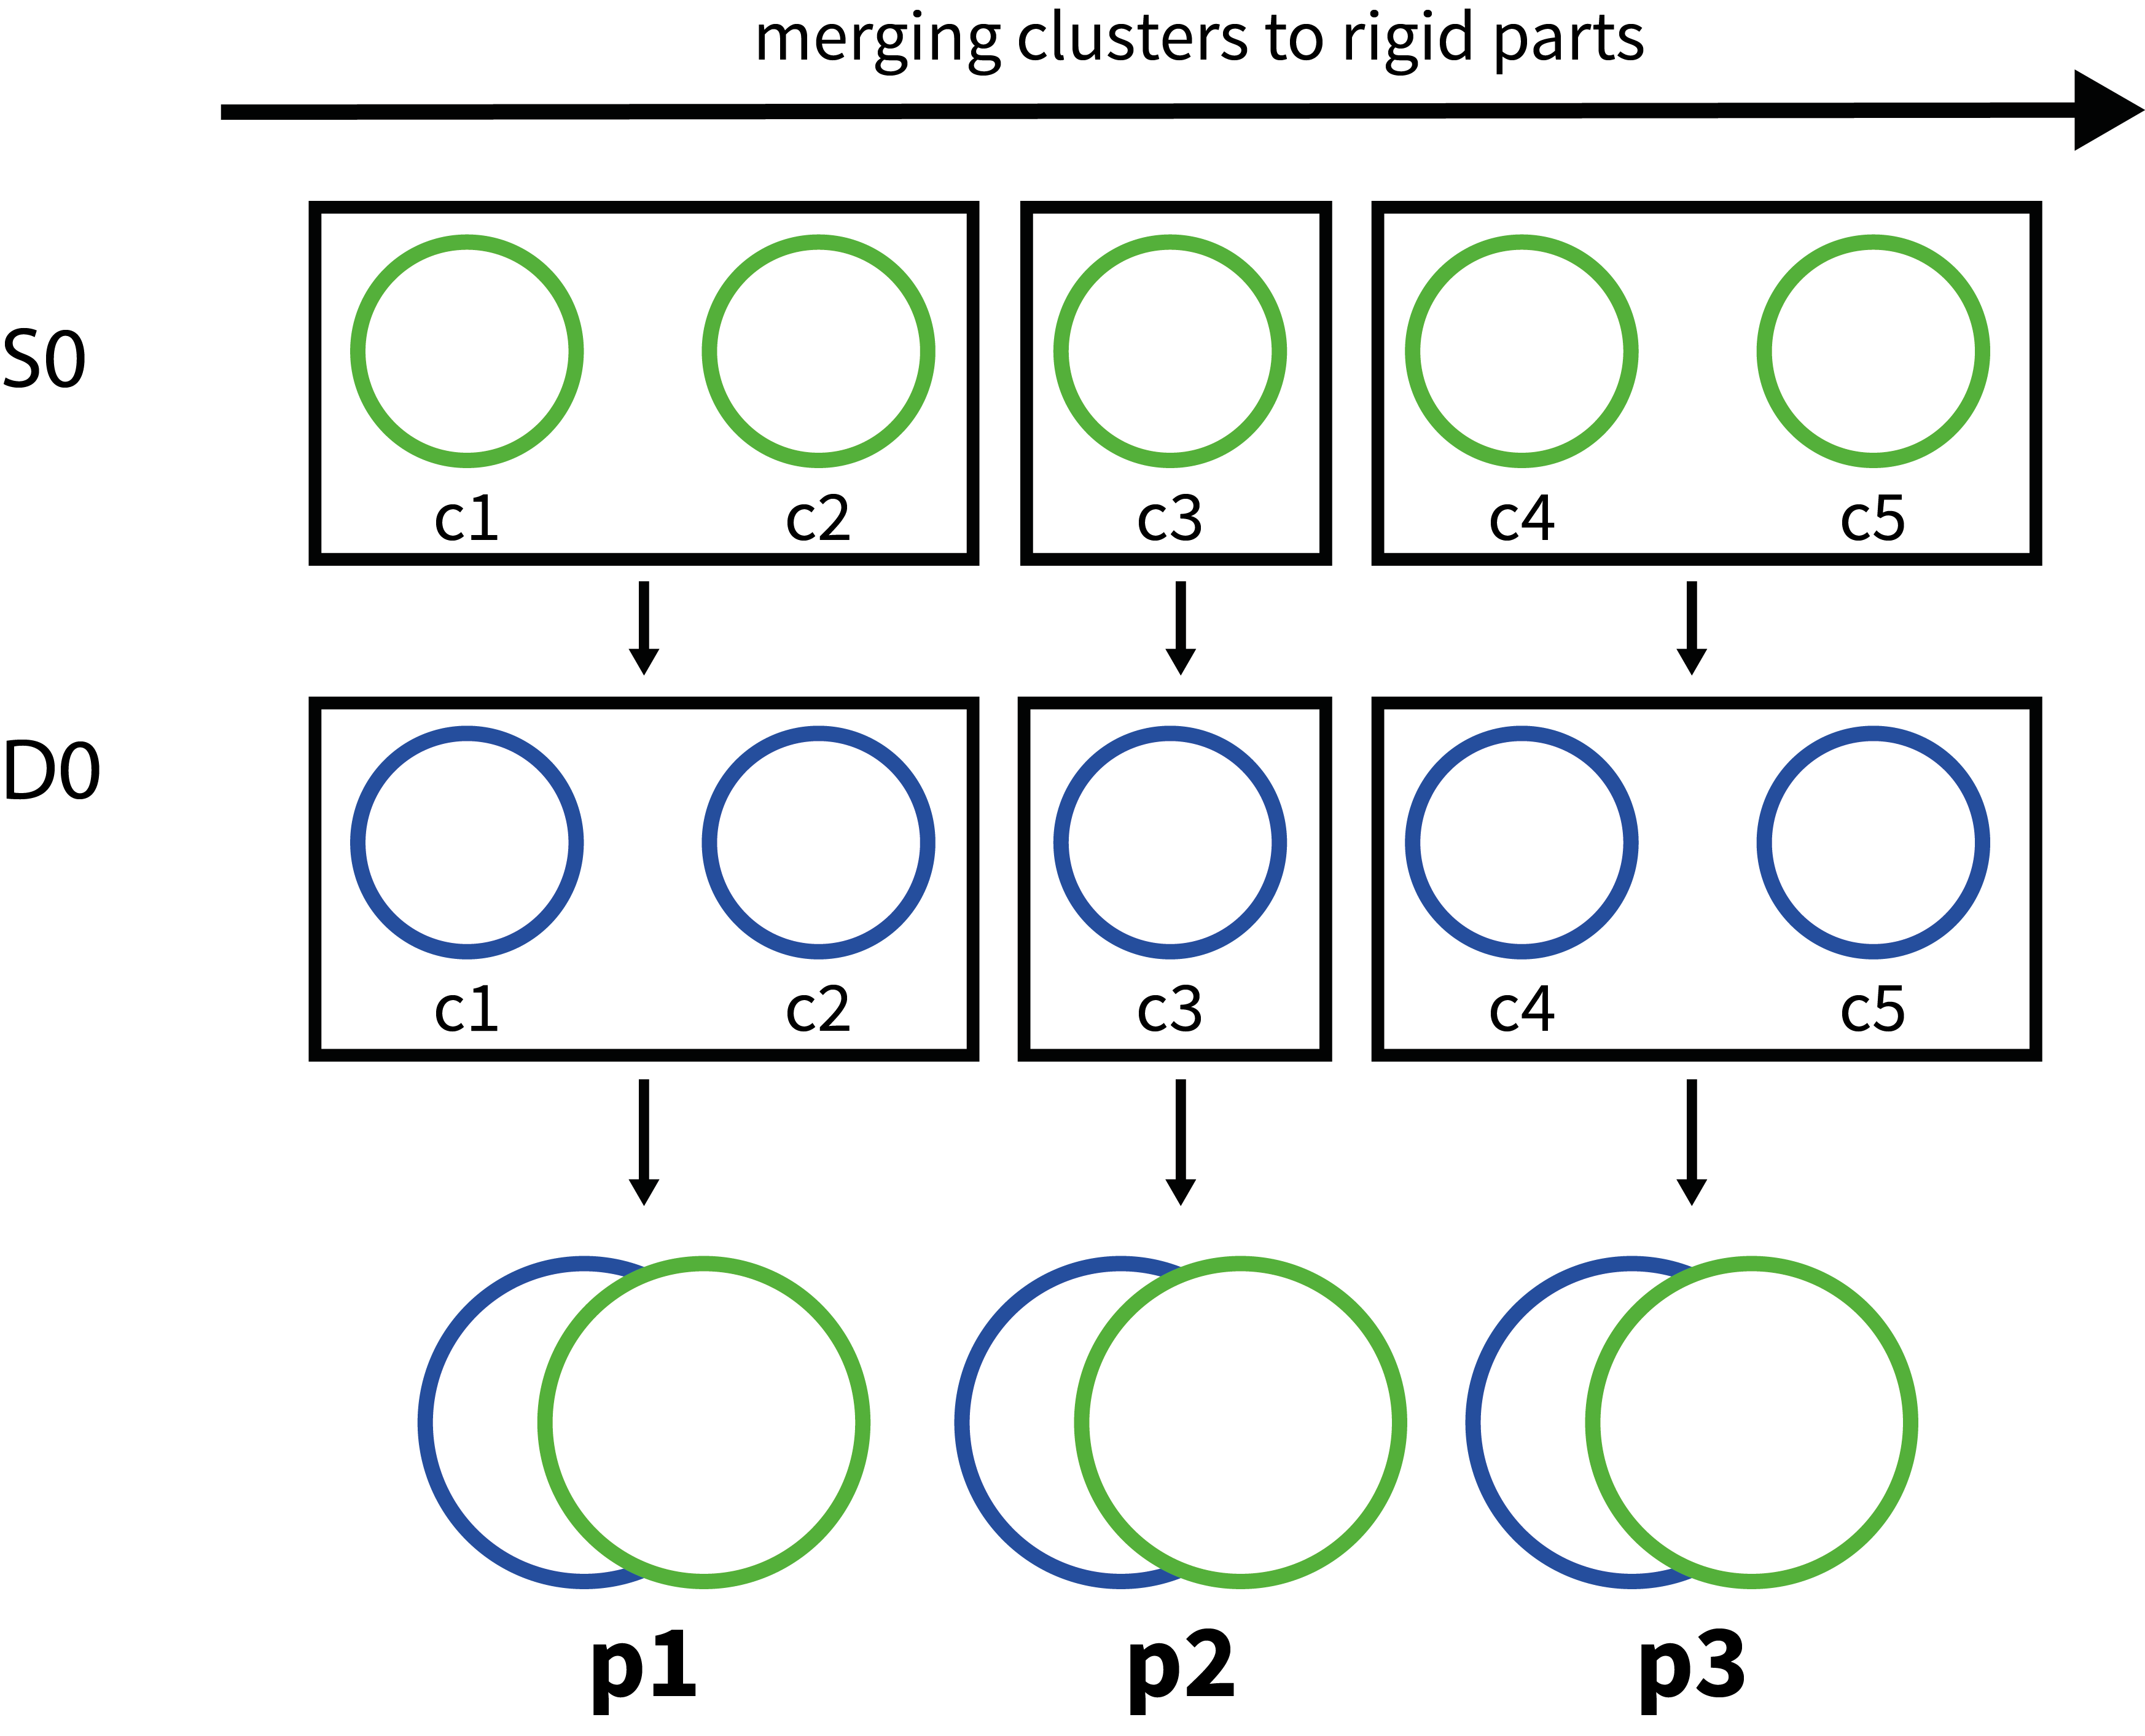
\includegraphics[width=0.7\linewidth]{ClusterChain}
	\caption{Detecting rigid parts of S0 and D0 by iteratively merging neighboring clusters of S0 and matching them with the merged clusters of DO. Genau erklären! }
	\label{fig:clusterChain}
\end{figure}

\subsection{Joint/skeleton estimation}

After detecting the rigid parts $ P =  \{ {p_1,....p_n}\}$, they are linked with joints and the principal axes are for now assumed to form the skeleton. 

\section{Implementation}

My approach was implemented in Java, using ImageJ as processing library, to focus on implementing and testing the algorithm in 2D. Another implementation is planned for 3D with the PCL to bring the attention to segmentation in 3D, and visualization. A class Cluster was implemented to store cluster points, its centroid, the orientation as well as the principal and secondary axes. For the subdividing, a cluster tree was implemented to simultainiously divide the initial clusters $c_{S, 0}$ and $c_{D, 0}$ into sub clusters \ref{subdividing}. Each node $N$ contains thereby two associated clusters $c_{S, i}$ and $c_{D, i}$. For the clustering and merging of clusters a List of Clusters was used to dynamically add and remove Clusters. Furthermore, a class ICP was created, which takes two clusters to be matched as input.

\subsection{Implementation Steps}

\begin{enumerate}
	\item The point clouds $S_0$ and $D_0$ are taken as input and clustering is computed to get the biggest clusters $cS_i$ = $cS_0$ and $cD_i$ = $cD_0$.
	
	\item The centroids $ctS_i$ and $ctD_i$ of $cS_i$ and $cD_i$ are computed.
	
	\item The principal axis $pS_i$ and $pD_i$ are computed through $ctS_i$ and $ctD_i$ in order to orient and align $cS_i$ and $cD_i$.
	
	\item The secondary axis $sS_i$ and $sD_i$ perpendicular to $pS_i$ and $pD_i$ through $ctS_i$ and $ctD_i$ are computed.
	
	\item The ICP between $cS_i$ and $cD_i$ and an error distance per point $e_{avg}$ are computed. 
	
	\item In case of $e_{avg} > \tau$, the dividers $dS_i$ and $dD_i$ to subdivide $cS_i$ and $cD_i$ are initialized with the secondary axis $sS_i$ and $sD_i$.
	
	\item The cluster points $ CP =  \{ {cp_0, ..., cp_n}\}$ of $cS_0$ and $cD_0$  are either allocated to $cS_{i + 1}$ or $cS_{i + 2}$ depending on its position $cp_i.x$ to $ctS_i.x$ and $ctD_i.x$. 
	
	\item The algorithm continues with $cS_i$ = $cS_{i + 1}$ from step 2.
	
	\item If $e_{avg} \le \tau$
	
	\item An error distance \textit{e\textsubscript{left}} and \textit{e\textsubscript{right}} is obtained. The part with the most error per point is assumed to be not rigid which gives back an indicator where to divide \textit{S\textsubscript{0}} and \textit{D\textsubscript{0}}.
	
	\item The dividers \textit{d\textsubscript{S}} and \textit{d\textsubscript{D}} are shifted to the direction of the highest error. To be continued from step 5 until the total error \textit{e\textsubscript{total}} doesn't get smaller.
\end{enumerate}



\subsection{Intermediate results}

At first, the implementation was tested on two point clouds of an articulated object with only two rigid parts. The segmentation results are directly dependent on the matching error threshold $\tau$ which can bee seen on table \ref{table:segmentation_results}. The higher the threshold $\tau$, the less clusters and subsequently rigid parts can be detected, as two clusters are more likely to match and are not further subdivided. The lower $\tau$, the more clusters and rigid parts will be detected, as clusters require further subdividing in order to match. Figure \ref{fig:results_2parts_4th} shows the clusters of the object after subdividing them with $\tau = 4$ and the final rigid parts, figure \ref{fig:results_3parts_5th} shows the result with three parts with $\tau = 5$. In case of $\tau = 3$ too many segments are detected, in case of $\tau = 1$ no segmentation is conducted (see Figure \ref{fig:dc_results_2p}). Figure XXX shows the two registered point clouds, in case of no segmentation and in case of a right detection of rigid parts.

Open Problems!

\begin{algorithm}
	\caption{Subdividing of clusters}\label{subdividing}
	\begin{algorithmic}[1]
		\Procedure{ClusterTree}{a}
		\State $j \gets j-1$.
		\EndProcedure
	\end{algorithmic}
\end{algorithm}

\begin{table}
	\centering\small
	\begin{tabular}{ |c|c|c|c| } 
		\hline
		Rigid parts & $\tau$ & detected clusters & detected rigid parts \\
		\hline
		2 & 10 & cell3 & cell4 \\ 
		& 5 & cell3 & cell4 \\
		& 4 & cell3 & cell4 \\
		& 3 & cell3 & cell4 \\
		& 1 & cell3 & cell4 \\
		\hline
		3 & 10 & cell3 & cell4 \\ 
		& 5 & cell3 & cell4 \\
		& 4 & cell3 & cell4 \\
		& 3 & cell3 & cell4 \\
		& 1 & cell3 & cell4 \\
		\hline
	\end{tabular}
	\caption{Segmentation results}
	\label{table:segmentation_results}
\end{table}

\begin{figure}[htbp]
	\centering\small
	\begin{tabular}{cc}
		\fbox{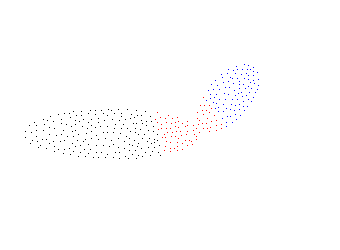
\includegraphics[width=0.45\textwidth]{2parts_clusters_4th}} &		% JPEG file
		\fbox{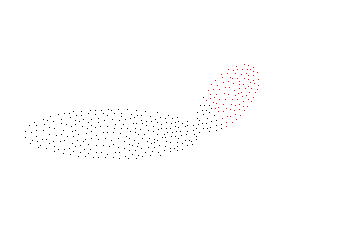
\includegraphics[width=0.45\textwidth]{2parts_rigidParts_4th}} 
		\\	% PNG file
		(a) & (b) 
	\end{tabular}
	\caption{Taking a mesh in two different poses as input (a), removing noise of the input point clouds (b)} 
	\label{fig:results_2parts_4th}
\end{figure}

\begin{figure}[htbp]
	\centering\small
	\begin{tabular}{cc}
		\fbox{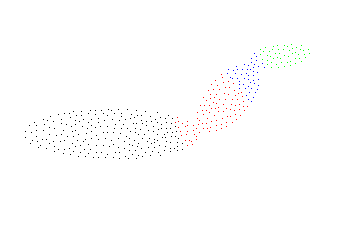
\includegraphics[width=0.45\textwidth]{3parts_clusters_5th}} &		% JPEG file
		\fbox{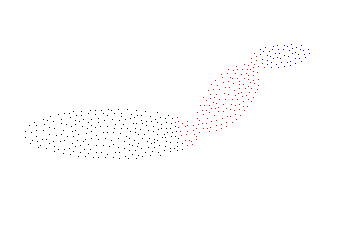
\includegraphics[width=0.45\textwidth]{3parts_rigidParts_5th}} 
		\\	% PNG file
		(a) & (b) 
	\end{tabular}
	\caption{Taking a mesh in two different poses as input (a), removing noise of the input point clouds (b)} 
	\label{fig:results_3parts_5th}
\end{figure}

\begin{figure}[htbp]
	\centering\small
	\begin{tabular}{cc}
		\fbox{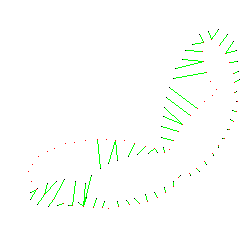
\includegraphics[width=0.45\textwidth]{3parts_associations_noSegmentation}} &		% JPEG file
		\fbox{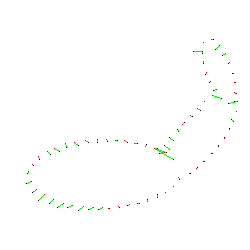
\includegraphics[width=0.45\textwidth]{3parts_associations_final}} 
		\\	% PNG file
		(a) & (b) 
	\end{tabular}
	\caption{Registration of two articulated objects before segmenting them into their rigid parts (a) and after the segmentation procedure (b). } 
	\label{fig:results_associations}
\end{figure}

The algorithm works satisfactory for simple objects, in which the rigid parts are aligned like in a chain. More complex object, e.g. a human, where one rigid part is linked to more than two rigid parts, improvements have to be implemented, for example detecting the largest rigid part and apply the algorithm for all remaining clusters (arms, legs). In case of dividing checking for multiple clusters, e.g. in case of a human.  Clusters not matching, as they don't have the same number of points, each point can only have one neighboring point. Or dividing clusters that they all have the same amount of points. In case of a more complex object where one rigid part can be linked with a high number of rigid parts (upper body of a humen) another approach has to be found, as the skeleton structure is different than from a chain. (see Figure \ref{fig:dc_results_2p}).

\subsection{Possible Improvements}

\subsubsection{LRP as initial alignment}

As only objects with rigid parts arranged like a chain are possible with this approach, another improvement/algorithm has to be pursued (see section \ref{sec:LRP}).

\subsubsection{Nearest neighbour}

Another improvement would be to ensure that each point only has one nearest neighbour and considering the case, that there are not always the same amount of points in two clusters. 

\subsubsection{Checking for multiple clusters}

Also a quite similar approach to \cite{guo2016correspondence}, in case of dividing or detecting a cluster, for the remaining clusters, region growing is conducted. 

\section{LRP}
\label{sec:LRP}

Instead of cutting the object initially in half, as an initial step the largest rigid part is found and recursively from there all other linked parts can be detected.

\subsection{Overview}
As an initial step, the LRP algorithm tries to find the most reliable correspondences, the so-called largest rigid part (LRP), subsequently all other parts are detected that are linked to the LRP. The initial alignment stage tries to find sparse correspondences between two point clouds by applying a single rigid transformation to detect the largest subsets of points in two point clouds. Starting from the LRP all other parts are detected recursively.

\subsection{Algorithm} 

\subsubsection{Finding the LRP}

The algorithm also takes two point clouds \textit{S\textsubscript{0}} and \textit{T\textsubscript{0}} of the same object in different configurations as input.
The goal is to find a single rigid transformation \textit{T\textsubscript{init}} for all points of \textit{S\textsubscript{0}} to get potential corresponding points \textit{C\textsubscript{0} = \{(s\textsubscript{i}, t\textsubscript{j})\}} in \textit{T\textsubscript{0}}. For that, local descriptors of \textit{S\textsubscript{0}} and \textit{T\textsubscript{0}} are computed. The requirement for a sparse correspondance between two points \textit{s\textsubscript{i}} and \textit{t\textsubscript{j}}  is that they are \textit{reciprocal}, which means that the Euclidean distance \textit{d(s\textsubscript{i}, t\textsubscript{j})} between them is the smallest in both directions. Some of the sparse correspondances are asumed to be wrong. Therefore, RANSAC is used on the sparse correspondances \textit{C\textsubscript{0}} to estimate a rigid alignment that is supported by the largest number of points \textit{n} from \textit{S\textsubscript{0}} and \textit{T\textsubscript{0}}. To assign the LRP in \textit{S\textsubscript{0}} and \textit{T\textsubscript{0}}, the biggest point clusters \textit{C\textsubscript{s}} and \textit{C\textsubscript{t}} of the overlapping area \textit{G\textsubscript{s} = \{C\textsubscript{1}, ... , C\textsubscript{n}\} } and \textit{G\textsubscript{t} = \{C\textsubscript{1}, ... , C\textsubscript{n}\} } are detected. 


\subsubsection{Part discovery}

The remaining clusters from \textit{S\textsubscript{0}} and \textit{T\textsubscript{0}} that have not been registered yet are matched recursively by starting with clusters connected to already matched parts. First, all matched parts are excluded from the input point clouds  \textit{G\textsubscript{s(l+1)}} = \textit{S\textsubscript{0}} - \textit{C\textsubscript{sl}} and \textit{G\textsubscript{t(l+1)}} = \textit{T\textsubscript{0}} - \textit{C\textsubscript{tl}} defining \textit{l} as the number of already matched parts \{1, ..., n\}, \textit{C\textsubscript{sl}}. For that clusters are formed, using region taking into account that they are attached to already registered parts. The algorithm explained is applied until all body parts have been discovered.

\subsection{Steps}

\begin{enumerate}
	\item The centroids \textit{c\textsubscript{s}} and \textit{c\textsubscript{t}} of \textit{S\textsubscript{0}} and \textit{T\textsubscript{0}} are computed.
	
	\item The principal axis \textit{p\textsubscript{s}} and \textit{p\textsubscript{t}}  are computed through \textit{c\textsubscript{s}} and \textit{c\textsubscript{t}} in order to horizontally orient the objects around their centroids.
	
	\item The ICP is conducted as a first guess to find a transformation \textit{T\textsubscript{init}} for all points from \textit{S\textsubscript{0}} that results in the highest number of corresponding points \textit{n} in \textit{T\textsubscript{0}}, given the threshold \textit{T}.
	
	\item \textit{C\textsubscript{0}} contains the corresponding points from S\textsubscript{0} and T\textsubscript{0}, resulting from \textit{T\textsubscript{init}(S\textsubscript{0})}.
	
	\item The RANSAC approach is applied on \textit{C\textsubscript{0}} to find a  \textit{T\textsubscript{f}} that results in the highest number of corresponding points \textit{n} between \textit{T\textsubscript{f}(S\textsubscript{0})} and \textit{T\textsubscript{0}}.
	
	\item The LRP is assigned to \textit{C\textsubscript{s}} and \textit{C\textsubscript{t}} from the resulting point clusters \textit{G\textsubscript{s}} and \textit{G\textsubscript{t}}.
	
	\item Starting from parts that are connected to the LRP, corresponding points \textit{C\textsubscript{i}} for unmatched points from \textit{S\textsubscript{0}} and \textit{T\textsubscript{0}} are seeked. The clusters are given as a input from Step 5. 
	
\end{enumerate}

\chapter{Conclusion}

In the beginning of the project, intense research was done in order to focus on one main problem. For that, it was quite essential to find the state-of-the-art regarding motion and pose estimation, in order to find a relevant topic as master thesis project. During research, the topic unsupervised pose estimation appeared. By focusing research in this direction, the non-rigid registration became a major indicator for possible optimizations. Taking existing methods as reference (see Chapter \ref{cha:relatedWork}), an own approach for 2D point clouds was developed, which should reduce the computation steps of detecting the rigd parts of an articulated non-rigid object. To do that, a divide-and-conquer approach was developed, which recurisively divides two point-clouds of the same object in different poses into matching clusters. The subdividing was realised with a tree and depth-first traversal to divide the point-clouds from left to right. As a next step all neighboring cluster were verified to be merged, in case of having subdivided a rigid part. After the mergin the rigid parts from left to right of the objects are detected. 

\section{Future work}

The focus in the next semester will be intensive testing of the current implementation and adding possible improvements. Eventually other existing approaches are taken into account to be able to segment more complex objects. The next main step is then, to implement the finished segmentation algorithm in 3D using the PCL. 


%%%----------------------------------------------------------
\MakeBibliography[nosplit]
%%%----------------------------------------------------------



\end{document}
